\documentclass[10pt]{beamer}

\usetheme[progressbar=frametitle]{metropolis}
\usepackage{graphicx}
\usepackage{appendixnumberbeamer}
\usepackage{booktabs}
\usepackage[scale=2]{ccicons}
\usepackage{pgfplots}
\usepgfplotslibrary{dateplot}
\usepackage{tabularx}
\usepackage{xspace}
\usepackage[utf8]{inputenc}
\usepackage{setspace}
\usepackage{pifont}% http://ctan.org/pkg/pifont
\usepackage{xcolor}
\definecolor{cmarkcolor}{RGB}{116, 209, 105}
\definecolor{xmarkcolor}{RGB}{230, 25, 25}
\newcommand{\cmark}{\color{cmarkcolor}\ding{51}}
\newcommand{\xmark}{\color{xmarkcolor}{\ding{55}}}%
\setbeamertemplate{bibliography item}[text]
\usepackage{minted}
\usepackage{multirow}
\usepackage{makecell}
 \newcolumntype{^}{>{\global\let\currentrowstyle\relax}}
%  \newcolumntype{}{>{\currentrowstyle}}
 \newcommand{\rowstyle}[1]{\gdef\currentrowstyle{#1}%
   #1\ignorespaces
 }
 \usepackage{animate}
 \usepackage{multimedia}
\usepackage{amsfonts,amssymb,amsthm,amsmath}
\newcommand{\themename}{\textbf{\textsc{metropolis}}\xspace}
\titlegraphic{
\includegraphics[height=1cm]{Logo-Exascale.png}}
\title{VeriTracer: Context-enriched tracer for floating-point arithmetic analysis}
\subtitle{ARITH 25, Amherst MA USA, June 2018}
% \date{}
\author{\underline{Yohan\,Chatelain}\inst{1,5} \and
    Pablo\,de\,Oliveira\,Castro\inst{1,5} \and
    Eric\,Petit\inst{2,5} \and
    David\,Defour\inst{3} \and 
    Jordan\,Bieder\inst{4,5} \and
    Marc\,Torrent\inst{4,5}}

\institute{%
\inst{1}Université de Versailles Saint-Quentin-en-Yvelines (UVSQ) \\
\inst{2}Intel \\
\inst{3}Université de Perpignan Via Domitia (UPVD) \\
\inst{4}CEA, DAM, DIF \\
\inst{5}Exascale Computing Research (ECR)
}

\setbeamersize{text margin left=20pt,text margin right=20pt}

\begin{document}

\maketitle
\begin{frame}{Table of contents}
  \setbeamertemplate{section in toc}[sections numbered]
  \tableofcontents[hideallsubsections]
\end{frame}

\section{Introduction}
\begin{frame}[fragile]{Context}
\metroset{block=fill}
\textbf{Building fast and robust applications for HPC is a complex task !}
\begin{figure}

\includegraphics[width=\linewidth]{numerical_chain.png}
\end{figure}
\begin{itemize}
\item At each step, numerical bugs can be introduced
\end{itemize} 
\textbf{\alert{Objective}: Tools to track and analyze numerical bugs}
\end{frame}

% \begin{frame}{Methods}
% \metroset{block=fill}
% \begin{alertblock}{Detects bugs}
% \begin{itemize}
% \item Formal: 
% \begin{itemize}
% \item Static analysis
% \item Abstract interpretation
% \item Interval arithmetic
% \end{itemize}
% \item Empirical:
% \begin{itemize}
% \item Extended Precision (EP)
% \item Stochastic methods
% \end{itemize}
% \end{itemize}
% \end{alertblock}
% \begin{alertblock}{Optimizes}
% \begin{itemize}
% \item Robustness:
% \begin{itemize}
% \item Formula rewriting
% \end{itemize}
% \item Performance:
% \begin{itemize}
% \item Mixed-precision
% \item Formula rewriting
% \end{itemize}
% \end{itemize}
% \end{alertblock}
% \end{frame}
% \begin{frame}[fragile]{Context}
% \metroset{block=fill}
% \textbf{Building fast and robust applications for HPC is a difficult task !}
% \begin{itemize}
% \item HPC systems
% \begin{description}
% \item[\textbullet] massive parallelism, asynchronicity, large SIMD vectors, complex memory hierarchy
% \item[$\Rightarrow$] tools for profiling time, memory, IO, optimizations (vectorization, memory placement, load unbalancing)
% \end{description}
% \item[] \textbf{Numerical simulations}
% \begin{itemize}
% \item complex multi-physics, high spatial and temporal resolution \newline
% $\Rightarrow$ strong mathematical background for centuries
% \end{itemize} 
% \item[] \textbf{Floating Point model}
% \begin{itemize}
% \item approximates real numbers, finite precision, loss of arithmetical properties, absorption, cancellation
% \item strong mathematical background ...
% \item ... but few tools for debugging/optimizing 
% \end{itemize}
% \end{itemize}
% \alert{\textbf{Needs tools for developing/debugging the floating-points problems in HPC environment}}
% \end{frame}
% \begin{frame}[fragile]{Existing tools}
% \begin{scriptsize} 
%  \begin{table}
%     \begin{tabular}{$c|^c^c^c$}
%       \toprule
%       \rowstyle{\bfseries}
%       \parbox[t]{2mm}{\multirow{8}{*}{\rotatebox[origin=c]{90}{Debugging}}} &
%       Method & Name & Implementation \\
%       \cmidrule{2-4}
%       & \multirow{3}{*}{\thead{Stochastic \\ Arithmetic}} & 
%       CADNA~\cite{jezequel2008cadna} & CESTAC/DSA  (library)   \\
%       && VERROU~\cite{fevotte2016verrou} & CESTAC  (Valgrind) \\
%       && Verificarlo~\cite{denis2016verificarlo} & MCA  (LLVM)  \\
%       \cmidrule{2-4}
% %       Veritracer & MCA & LLVM & \cmark & asynchronous \\
%       & \multirow{4}{*}{\thead{Extended \\ Precision \\ (EP)}} & 
%       HPC Craft~\cite{lam2013dynamic} & Exponent comparison  (DynInst)  \\
%       && FpDebug~\cite{benz2012dynamic} & MPFR  (Valgrind)  \\
%       && Herbgrind~\cite{sanchez2017finding} & MPFR  (Valgrind)   \\
%       && &  \\
%       \bottomrule
%     \end{tabular}
%   \end{table}
%   \begin{center}
%   % 	\begin{tabularx}{\linewidth}{$c|^l^l^c^c^l}
% 	\begin{tabular}{$c|^c^c^c^c$}
%       \toprule
%       \rowstyle{\bfseries}
%       \parbox[t]{2mm}{\multirow{6}{*}{\rotatebox[origin=c]{90}{Optimization}}} &
%       Name & Method & Mixed-Precision & Any-Precision \\
%       \cmidrule{2-5}
%       & Verificarlo~\cite{denis2016verificarlo} & MCA (User specific) & \cmark & \cmark  \\
%       & HPC Craft~\cite{lam2013dynamic} & Bitmask (ref value) & \cmark  & \cmark   \\
%       & Promise~\cite{graillat:hal-01331917} & CESTAC/DSA ($\Delta-debug$) & \cmark  & \xmark  \\
%       & Precimonious~\cite{rubio2013precimonious}& EP ($	\Delta-debug$) & \cmark & \xmark  \\ 
%       & Herbie~\cite{panchekha2015automatically} & EP (Rewriting) & \xmark & \xmark  \\
% 	\bottomrule
%     \end{tabular}
% \end{center}
% \end{scriptsize}
% \end{frame}

\begin{frame}[fragile]{Muller's sequence\cite{bajard1996introduction} overview}
\metroset{block=fill}
\begin{small}
% \begin{alertblock}{Muller's sequence~\cite{bajard1996introduction}}
% \begin{center}
% $\mathbf{u_{n+1} = 111 - \dfrac{1130}{u_{n}} + \dfrac{3000}{u_{n}u_{n-1}}}$
% \end{center}
% \vspace{-.4cm}
% With initial conditions $u_0 = 2$ and $u_1 = -4$
% \vspace{-.2cm}
% \begin{itemize}
% \item When computing the~~\alert{exact solution}~~~$\Rightarrow \lim=6$
% % \lim_{n \to \infty}u_n=6$
% \item When computing with \alert{finite precision} $\Rightarrow \lim =100$
% % \lim_{n\to\infty}u_n=100$
% \end{itemize}
% \end{alertblock}

\begin{figure}
\only<1>{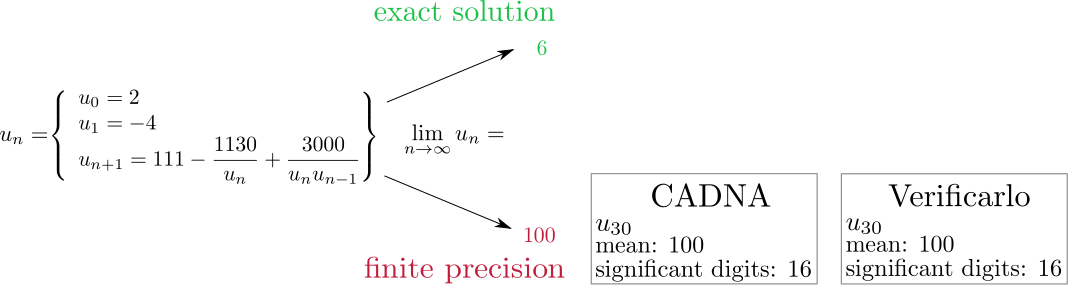
\includegraphics[width=\linewidth]{muller.png}}
\only<2>{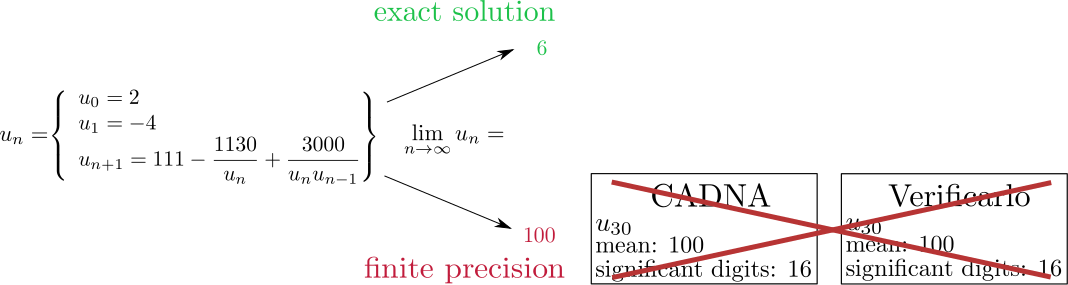
\includegraphics[width=\linewidth]{muller_2.png}}
\end{figure}

\only<1>{Stochastic methods execute several samples by introducing random errors}
% \alert{Value of $u_{30}$}
% \begin{tabular}{|l|l|l}
% Tool & Mean & Number of significant digits \\
% \toprule
% CADNA & 0.100000000000000E+003 & 16\\
% \midrule
% Verificarlo & 1.0000000000000000E+02 & 16 \\
% \end{tabular}
\only<2>{
\begin{alertblock}{Without an exact solution}
\begin{itemize}
% \item One can conclude that the computation is fully \alert{precise}
% \item In this case, however, the calculation is \alert{precisely wrong} 
\item Only checking the final result may leads to wrong conclusions !
\end{itemize}
\end{alertblock}
}
\end{small}
\end{frame}

\begin{frame}{Current challenges}
Existing tools explore the \alert{spatial} dimension of numerical computations:
\begin{itemize}
\item which variable or operation is imprecise
\item which function can be switched into lower precision
\item but programs have different numerical requirements over time
\end{itemize}
% \begin{figure}
% 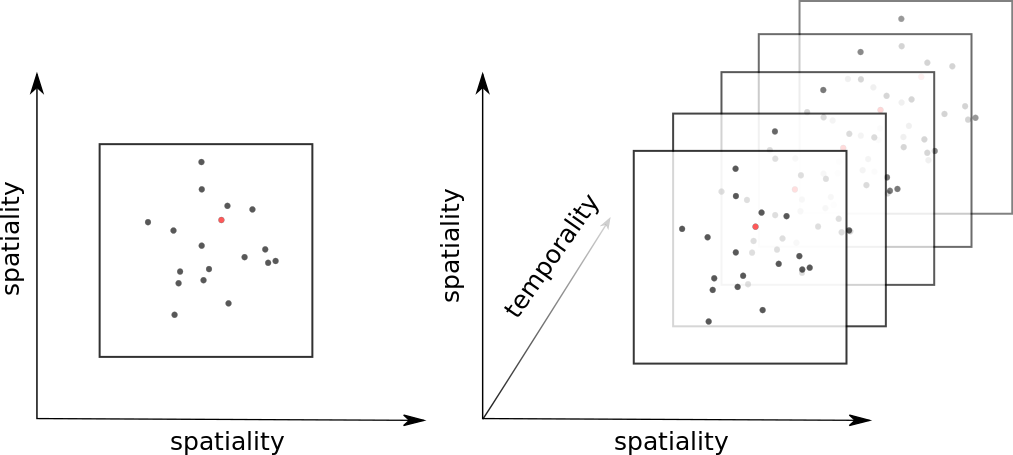
\includegraphics[width=.9\linewidth]{space-time.png}
% \end{figure}
\begin{center}
\begin{large}
$\Rightarrow$ \textbf{Need to explore the \alert{temporal} dimension}
\end{large}
\end{center}
\end{frame}

\section{Veritracer}

\begin{frame}[fragile]{Instrumentation}
\metroset{block=fill}
\begin{alertblock}{Veritracer LLVM pass}
\begin{itemize}
\item Accepts any source code accepted by the LLVM frontend
\item Transforms into an LLVM Intermediate Representation
\item Searches debug information through LLVM IR
\item Instruments the IR code with veritracer probes
\end{itemize}
\end{alertblock}
\begin{figure}
% 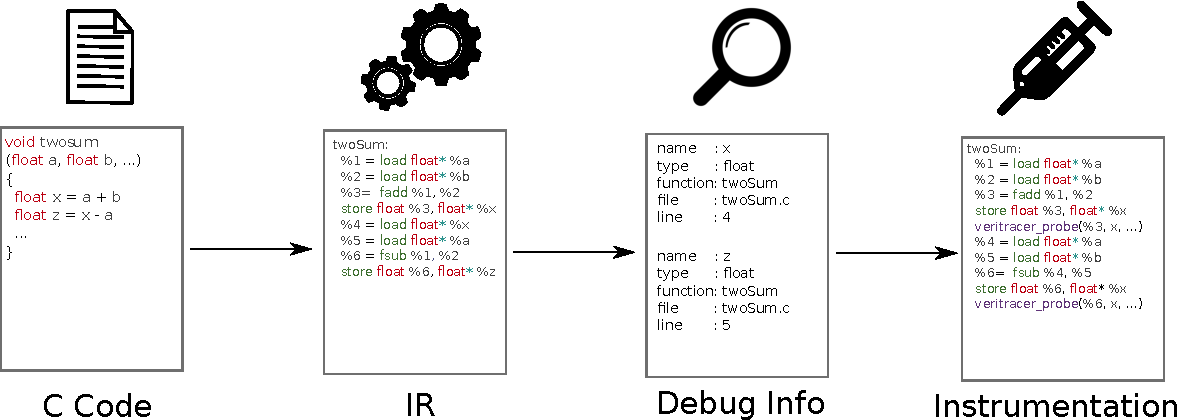
\includegraphics[width=\linewidth]{llvm_flow.pdf}
\end{figure}
\end{frame}

\begin{frame}{Information Flow Analysis}
\metroset{block=fill}
\begin{alertblock}{Ansychronous analysis}
\begin{itemize}
\item Veritracer works in an asynchronous way
\item Information flow is necessary for gathering the traces
\item Three levels of granularities are analyzed:
\begin{itemize}
\item \textbf{Context Analysis}: considers the context of a function call
\item \textbf{Control-Flow Analysis}: considers the flow path taken
\item \textbf{Data-Flow Analysis}: considers the dependencies between variables
\end{itemize}
\end{itemize}
\end{alertblock}
\begin{figure}
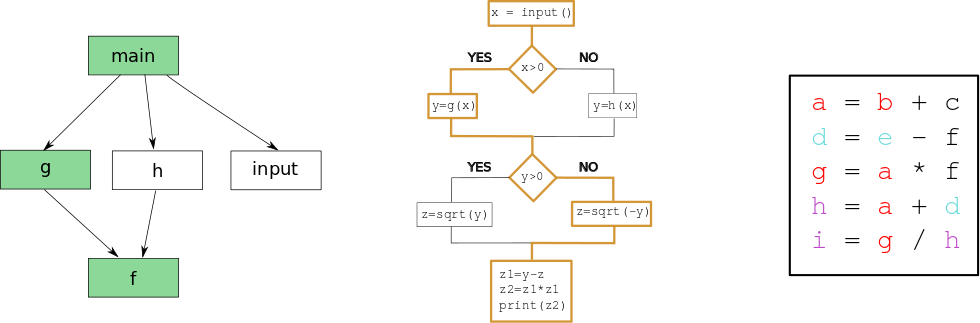
\includegraphics[width=\linewidth]{IFA.png}
\end{figure}
\end{frame}

\begin{frame}{Pinpointing relevant function}
\metroset{block=fill}
\begin{alertblock}{Narrowing the search space}
To narrow the search space, we:
\begin{description} 
\item[Scan] functions with FP values
\item[Narrow] the set by removing
non-contributing functions \newline $f_{{\delta e}_{\max}}(x) \leq \epsilon, $
\item [Order] functions by \textit{numerical stress resistance} \newline $\min_{\delta e} \{ f_{{\delta e}_{\min}} \leq \epsilon \}$
\end{description}
\end{alertblock}
\vspace{-.4cm}
\begin{figure}
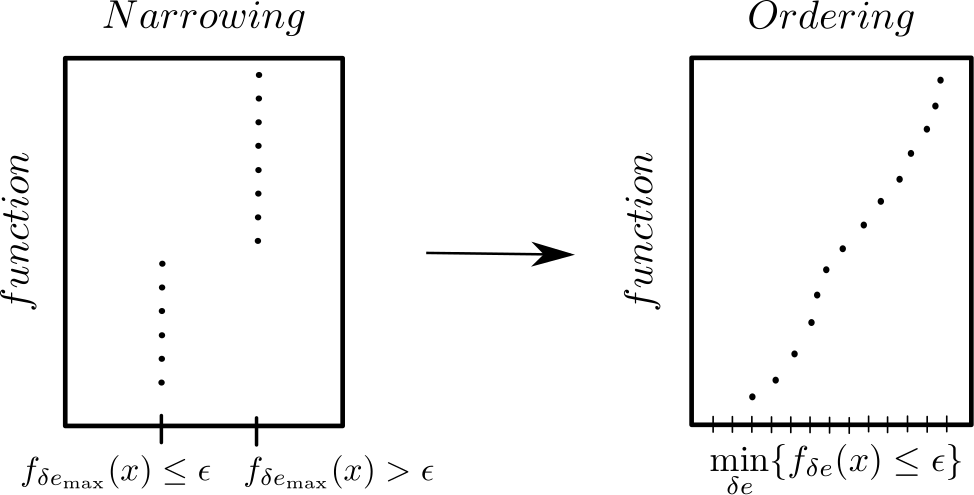
\includegraphics[scale=.25]{pinpointing_2.png}
\end{figure}
\end{frame}

\begin{frame}[fragile]{Implementation}
\metroset{block=fill}
\vspace{.2cm}
\begin{alertblock}{Extends verificarlo to}
\begin{itemize}
\item Trace the precision of FP variables \alert{over time}
\item Provide \alert{contextual information} on traced variables
\begin{itemize}
\item Current version implements Context Analysis
\item Inserts call to \texttt{backtrace()} (GNU C library)
\item Analyzes backtraces to detect flow divergences
\end{itemize}
\item \alert{All in an automatic way}
\end{itemize}
\end{alertblock}
\begin{figure}
\vspace{-0.25cm}
\noindent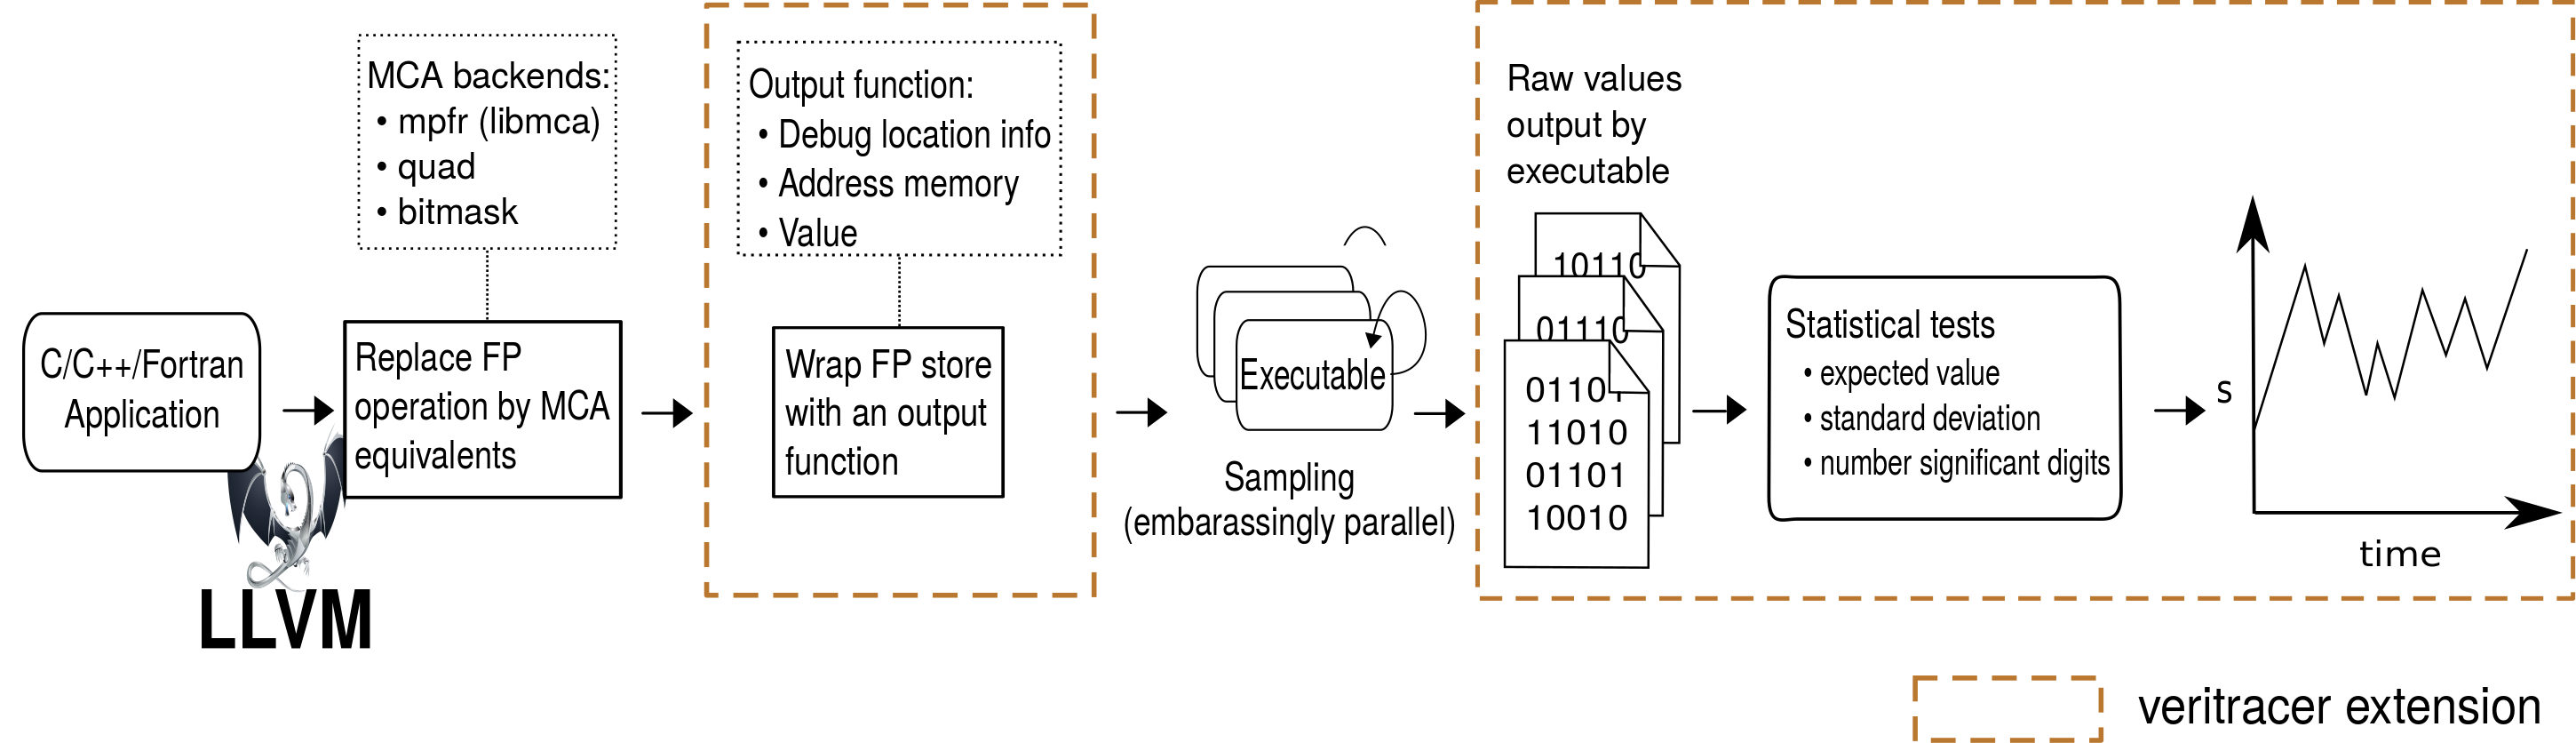
\includegraphics[width=\linewidth]{veritracer_workflow_line2_dash.png}
\caption{Veritracer's workflow}
\end{figure}
\end{frame}



\begin{frame}[fragile]{Monte Carlo Arithmetic (MCA)~\cite{parker1997monte}}
	\metroset{block=transparent}
    \vspace{.2cm}
 \begin{alertblock}{$ \mathbf{inexact(x) = x + \beta^{e_x-t}\xi} $}
  \begin{itemize}  
  \item $e_x$ is the magnitude of $x$
  \item $t$ the virtual precision
  \item $\xi$ a random variable between $\left]-\frac{1}{2},\frac{1}{2}\right[ $
  \end{itemize}
  \end{alertblock}
	 \metroset{block=fill}
  \begin{alertblock}{Random Rounding mode }
	\begin{itemize}
	\item $RR(x \circ y) = inexact(x \circ y),~\circ \in \{+,-,\times, \backslash\} $ 
    \end{itemize}       
  \end{alertblock}
   \begin{figure}
  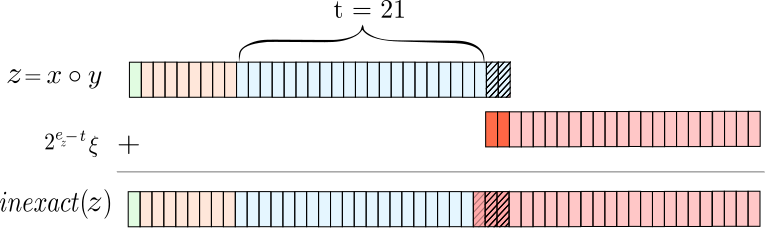
\includegraphics[width=\linewidth]{mca_model_RR__line.png}
  \end{figure}
% \begin{alertblock}{Three modes for adding errors}
% \begin{itemize}
% \item Random Rounding: $RR(x) = inexact(x \circ y)$
% \begin{itemize}
% \item \alert{Simulates roundoff errors}
% \end{itemize}
% \item Precision Bounding: $PB(x) = inexact(x) \circ inexact(y)$
% \begin{itemize}
% \item \alert{Detects cancellations}
% \end{itemize}
% \item Full MCA: $MCA(x) = inexact(inexact(x) \circ inexact(y))$
% \begin{itemize}
% \item \alert{Composition of RR and PB modes}
% \end{itemize}
% \end{itemize}
% \hspace{.5cm} with $ \circ \in \{+,-,\times, \backslash\}$
% \end{alertblock}
\end{frame}



% \begin{frame}[fragile]{Muller's sequence with veritracer}
% \begin{figure}
% 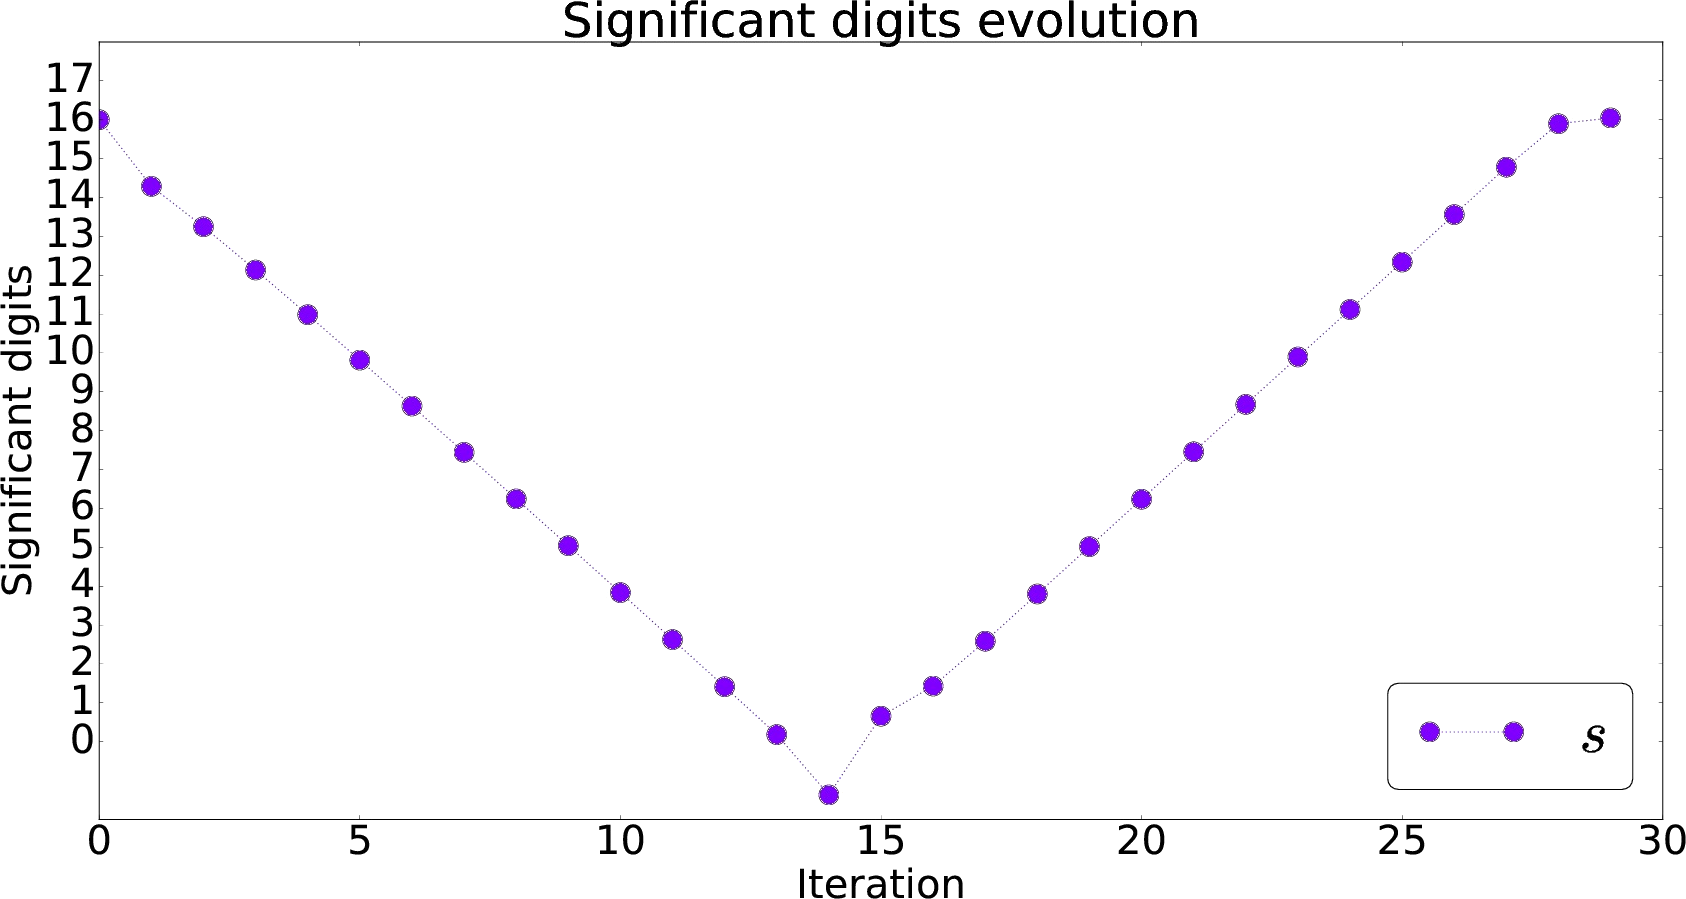
\includegraphics[width=.8\linewidth]{muller_sequence.png}
% \caption{Muller's sequence evaluation over 500 samples with verificarlo.
% Evolution of the number of significant digits of $u_n$ over time. \newline
% Compiled with double format and executed with $t=53$ in RR mode}
% \end{figure}
% \begin{itemize}
% \item Automatically plots the number of significant digits over time
% \item At $n=14$ there are no more significant digits correct
% \end{itemize}

% \end{frame}

% \section{Information Flow Analysis}

% \begin{frame}{Information Flow Analysis}
% \metroset{block=fill}
% \begin{alertblock}{Information flow analysis}
% Detects how information is propagated through an application
% \end{alertblock}
% \end{frame}

% \begin{frame}{Information Flow Analysis}
% \metroset{block=fill}
% \begin{minipage}{0.55\linewidth}
% \begin{block}{Three granularities}
% \begin{itemize}
% \item \alert{\textbf{Context Analysis}}: considers the context of a function call
% \item \textbf{Control-Flow Analysis}: considers the flow path taken
% \item \textbf{Data-Flow Analysis}: considers the dependencies between variables
% \end{itemize}
% \end{block}
% \end{minipage}
% \hspace{.25cm}\begin{minipage}{0.4\linewidth}
% \only<1>{
\includegraphics[width=\linewidth]{context.png}}
% \only<2>{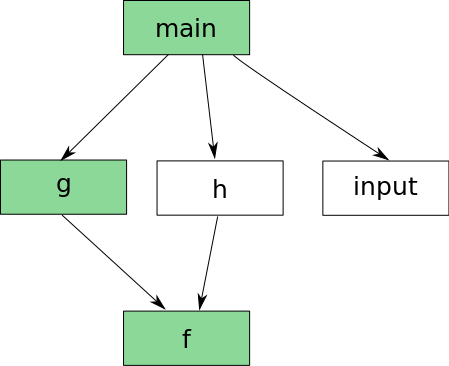
\includegraphics[width=\linewidth]{context_CSP1.png}}
% \only<3>{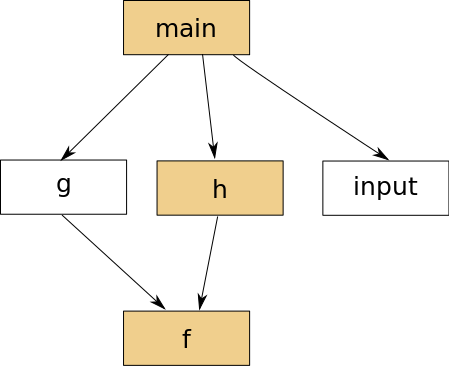
\includegraphics[width=\linewidth]{context_CSP2.png}}
% \end{minipage}
% \end{frame}

% \begin{frame}{Information Flow Analysis}
% \metroset{block=fill}
% \begin{minipage}{0.55\linewidth}
% \begin{block}{Three granularities}
% \begin{itemize}
% \item \textbf{Context Analysis}: considers the context of a function call
% \item \alert{\textbf{Control-Flow Analysis}}: considers the flow path taken
% \item \textbf{Data-Flow Analysis}: considers the dependencies between variables
% \end{itemize}
% \end{block}
% \end{minipage}
% \hspace{.25cm}\begin{minipage}{0.4\linewidth}
% \only<1>{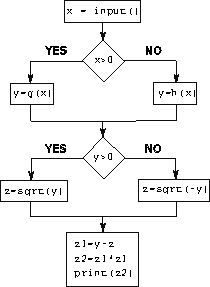
\includegraphics[width=.9\linewidth]{control.pdf}}
% \only<2>{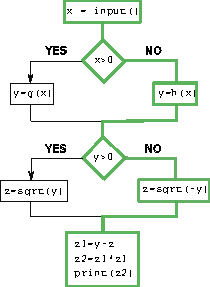
\includegraphics[width=.9\linewidth]{control_path1.pdf}}
% \only<3>{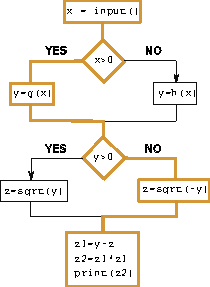
\includegraphics[width=.9\linewidth]{control_path2.pdf}}
% \end{minipage}
% \end{frame}

% \begin{frame}{Information Flow Analysis}
% \metroset{block=fill}
% \begin{minipage}{0.55\linewidth}
% \begin{block}{Three granularities}
% \begin{itemize}
% \item \textbf{Context Analysis}: considers the context of a function call
% \item \textbf{Control-Flow Analysis}: considers the flow path taken
% \item \alert{\textbf{Data-Flow Analysis}}: considers the dependencies between variables
% \end{itemize}
% \end{block}
% \end{minipage}
% \hspace{.25cm}\begin{minipage}{0.4\linewidth}
% \only<1>{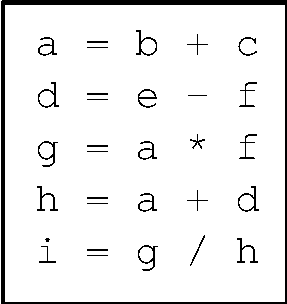
\includegraphics[width=.9\linewidth]{dataflow.pdf}}
% \only<2>{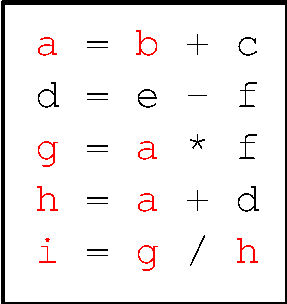
\includegraphics[width=.9\linewidth]{dataflow_red.pdf}}
% \only<3>{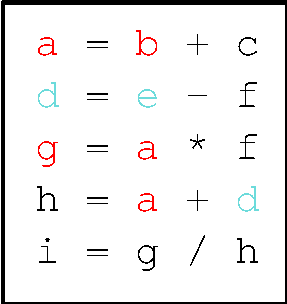
\includegraphics[width=.9\linewidth]{dataflow_blue.pdf}}
% \only<4>{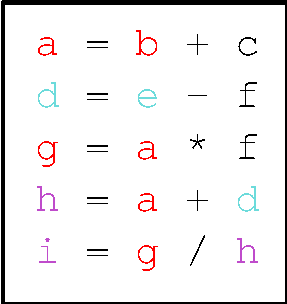
\includegraphics[width=.9\linewidth]{dataflow_violet.pdf}}
% \end{minipage}
% \end{frame}

% \begin{frame}{Current implementation status}
% \metroset{block=fill}
% \begin{alertblock}{Information Flow Analysis}
% Current version implements the Context Analysis:
% \begin{itemize}
% \item Inserts call to \texttt{backtrace} (GNU C library)
% \item Analyzes backtraces to detect flow divergences
% \item Each flow is plotted separately
% \end{itemize}
% \end{alertblock}
% \end{frame}
% \begin{frame}{Context Analysis}
% \metroset{block=fill}
% \begin{alertblock}{Context Analysis}
% Context-analysis considers the context of a function call 
% \begin{itemize}
% \item A function can be called by different parent
% functions 
% \item which can be called themselves by different
% functions... 
% \item The list of the caller ancestors is the Call
% Site Path (CSP)
% \item Depending on its CSP, a function may
% have different behaviors.
% \end{itemize}
% \end{alertblock}
% \begin{alertblock}{Solution}
% \begin{itemize}
% \item Maintains a stack of the CSPs (backtrace)
% \end{itemize}
% \end{alertblock}
% \end{frame}

% \begin{frame}{Control-Flow Analysis}
% The control-flow analysis considers the path taken within a function.
% \begin{figure}
% \begin{minipage}{0.4\linewidth}
% \includegraphics[width=.75\linewidth]{branchesV.png}
% \end{minipage}
% \begin{minipage}{0.5\linewidth}
% \begin{itemize}
% \item \textbf{Stage 1}: the program can take the branch 2 or not \\
% $\mathbf{\Rightarrow}$ The different execution traces will not exhibit the same number of variables traced, whether they take this branch or not
% \item \textbf{Stage 4,5}: both blocks use the
% same variables but in different sequences of operation \\
% $\mathbf{\Rightarrow}$ The different execution traces will not exhibit the same numerical quality even if the semantics are the same
% \end{itemize}
% \end{minipage}
% \end{figure}
% \end{frame}

% \begin{frame}{Control-Flow Analysis}
% \metroset{block=fill}
% \begin{alertblock}{The control-flow analysis considers the path taken within a function}
% \begin{minipage}{0.4\linewidth}
% \textbf{Stage 1}: the program can take the branch 2 or not
% \vspace{1mm}
% \hrule
% \vspace{1mm}
% $\mathbf{\Rightarrow}$ The different execution traces will not exhibit the same number of variables traced, whether they take this branch or not
% \end{minipage}
% \hspace{.75cm}
% \begin{minipage}{0.45\linewidth}
% \textbf{Stage 4,5}: both blocks use the
% same variables but in different sequences of operation
% \vspace{1mm}
% \hrule
% \vspace{1mm}
% $\mathbf{\Rightarrow}$ The different execution traces will not exhibit the same numerical quality even if the semantics are the same
% \end{minipage}
% \end{alertblock}
% \begin{figure}
% \includegraphics[width=.8\linewidth]{branches.png}
% \end{figure}
% \end{frame}

% \begin{frame}{Data-Flow Analysis}
% \metroset{block=fill}
% \begin{alertblock}{Data-Flow Analysis}
% The data-flow analysis considers the dependencies between variables across a program
% \begin{itemize}
% \item The errors introduced by MCA can be propagated through calculations
% \item Interesting to keep track of these dependencies
% \item Allowing to observe the interactions between variables
% \item Having information on errors propagation.
% \end{itemize}
% \end{alertblock}
% \end{frame}

% \begin{frame}{Data-Flow Analysis}
% \metroset{block=fill}
% \begin{alertblock}{Two solutions}
% \begin{itemize}
% \item \alert{\textbf{Taint-Analysis}}
% \begin{itemize}
% \item Checks which computations are affected by a set of variables. 
% \item A \alert{taint policy} defines the propagation rules for tainting.
% \item The \alert{taint flow} follows variables
% affected by the tainted variables
% \item Constructs the \alert{contamination chain} which represents the variables
% affected by the error introduced
% \end{itemize}
% \item \alert{\textbf{Forward symbolic execution}}
% \begin{itemize}
% \item Represents the execution of a program with a \alert{logical formula} 
% \item Possible to apply mathematical logic to the data-flow analysis
% \item Reasons on values domain providing strong proofs
% \item However, the number of possibilities to explore is \alert{exponential} !
% \end{itemize}
% \end{itemize}
% \end{alertblock}
% \end{frame}

\section{Experiments}

\subsection{Muller's sequence}

\begin{frame}{Muller's sequence with veritracer}
\begin{figure}
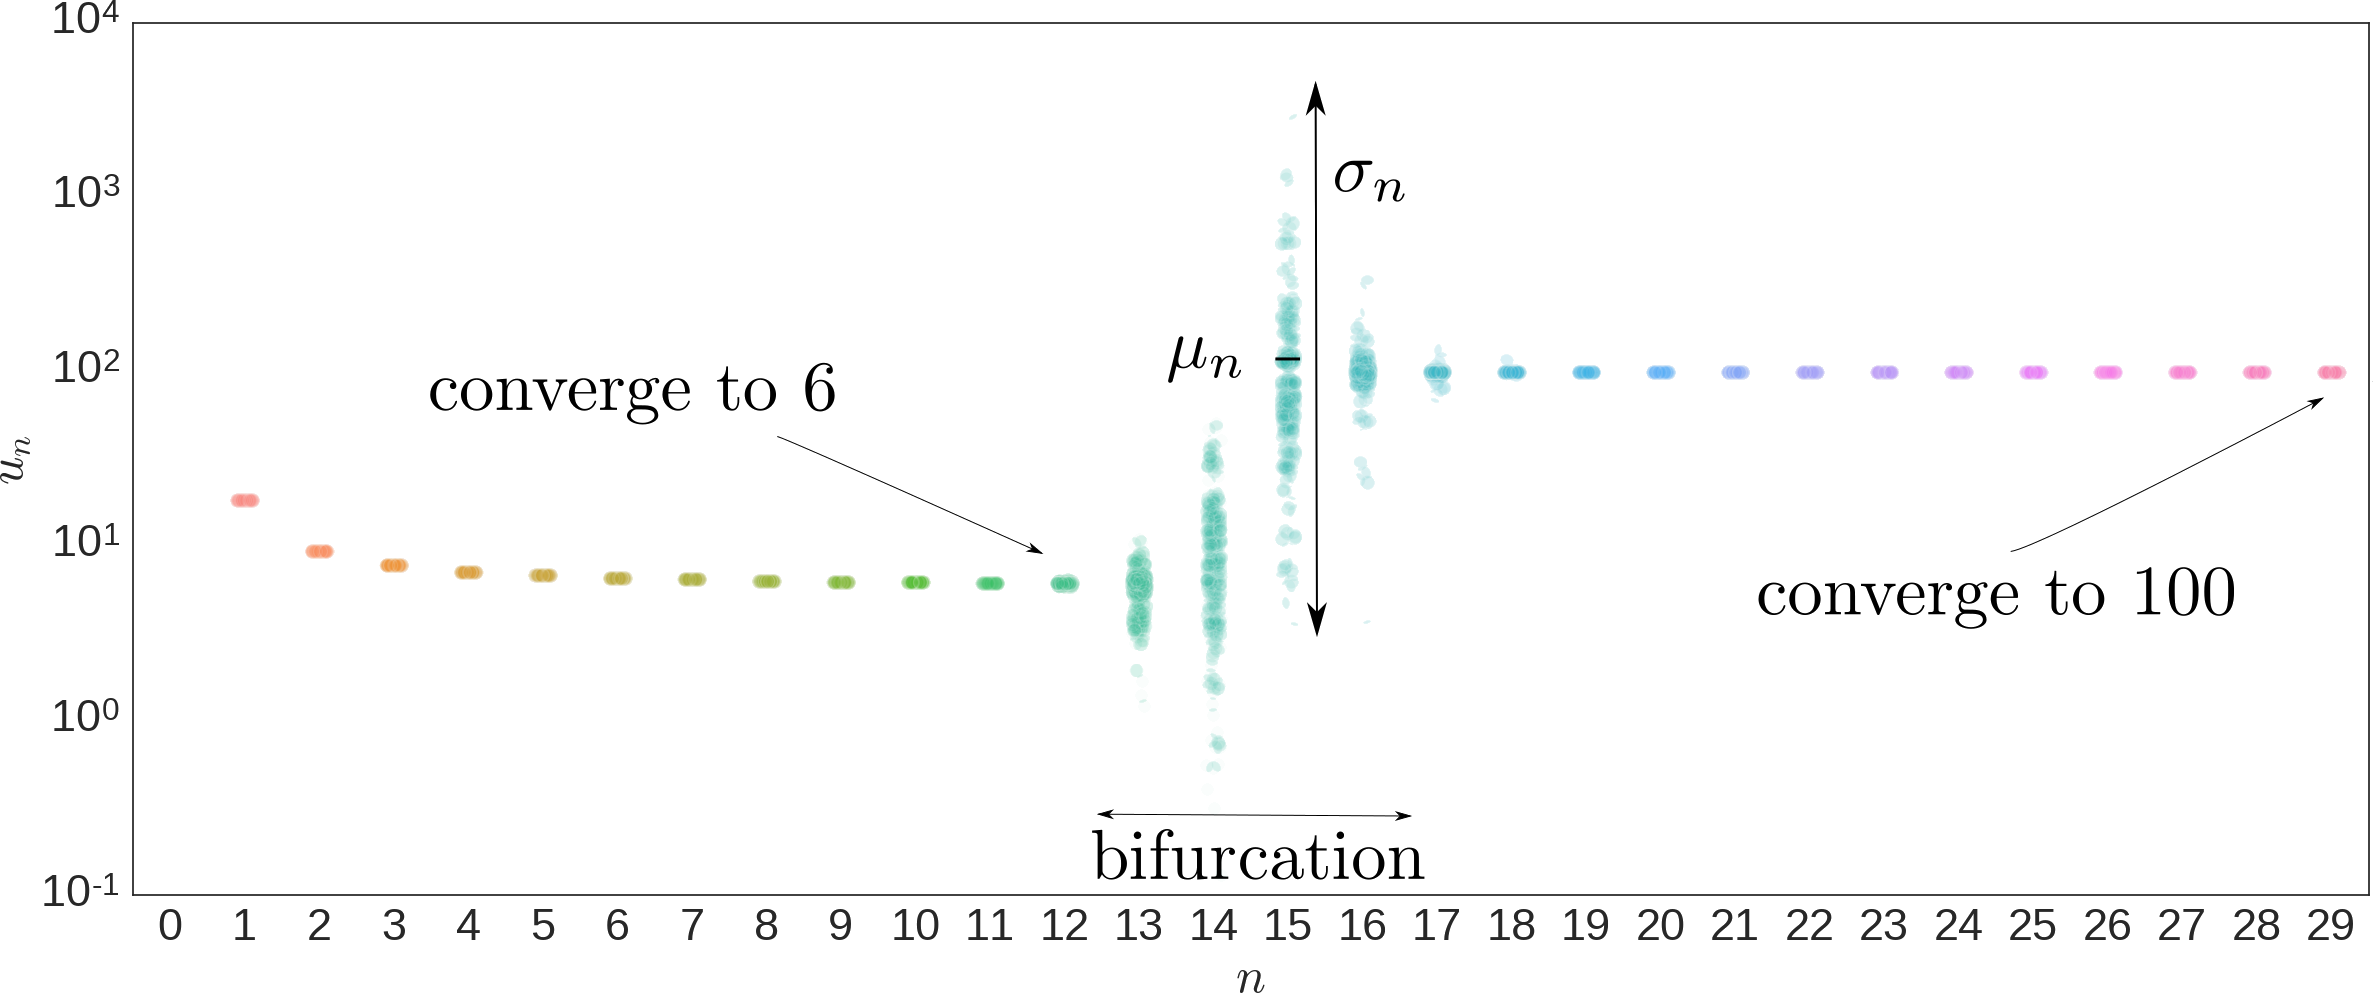
\includegraphics[width=\linewidth, height=4.5cm]{muller_jitter_annotated.png}
\caption{Muller's sequence evaluation over 500 samples with veritracer.
The sequence converges to 6 before bifurcating and then converges to 100.}
\end{figure}
\begin{itemize}
\item Estimate the number of significant digits by using N samples 
$\alert{\tilde{s} = - \log_{10} \left(\dfrac{\tilde{\sigma}}{\tilde{\mu}}\right)}$
\item $\alert{\tilde{\mu}}$: empirical mean and $\alert{\tilde{\sigma}}$: empirical standard deviation
\end{itemize}
\end{frame}

\begin{frame}[fragile]{ABINIT}
\metroset{block=fill}
\begin{footnotesize}
\begin{alertblock}{ABINIT~\cite{gonze2016recent} }
\begin{itemize}
\item Calculates observable properties of materials 
(optical, mechanical, vibrational)
% \item Uses quantum equations of \alert{Density Functional Theory (DFT)}
\item Works on \alert{any chemical composition} (molecules, nanostructures, solids)
\end{itemize}
\end{alertblock}
% \begin{alertblock}{The Perovskite use case}
% \begin{itemize}
% \item Computes the \alert{total-energy} of a system composed of 5 atoms ($BaTiO_3$) 
% \item Variant of a type of \alert{crystal structure} called Perovskite. 
% \item \alert{Deterministic computation}: same inputs = same results (IEEE)
% \end{itemize}
% \end{alertblock}
\begin{figure}
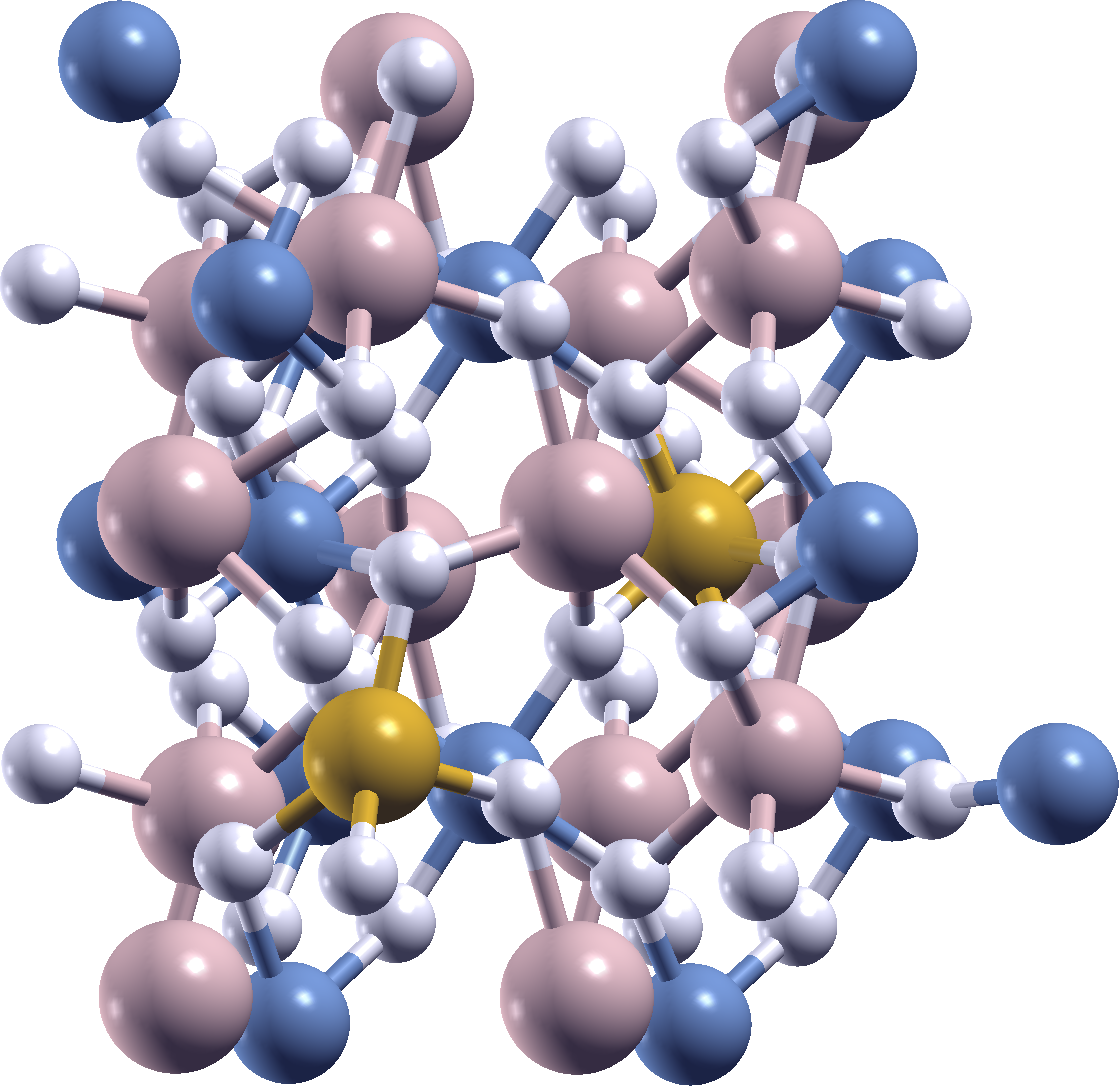
\includegraphics[width=5cm, height=5cm]{mgsio3_al.png}
\caption{Sound velocity calculation in an earth mantle component \newline ($MgSiO_3$ perovskyte with Al impurities)~\cite{ABINIT:siliconCarbide}}
\end{figure}
\end{footnotesize}
\end{frame}

% \metroset{block=fill}
% \begin{frame}[fragile]{Pinpointing relevant functions}
% \begin{alertblock}{Pinpointing relevant functions}
% Pinpointing relevant functions that have an impact on the numerical stability of the code
% leads to computational issues:
% \begin{itemize}
% \item Introducing MCA errors and tracing each function
% of a large code is an \alert{expensive process}
% \item Disturbing the computation of a function \alert{may impact
% the computation of others functions} 
% \item Analyzing all the possibilities leads to a \alert{combinatorial explosion}
% \end{itemize}
% \end{alertblock}
% \begin{alertblock}{Reducing the search space}
% To reduce the search space, we propose a two steps heuristic:
% \begin{enumerate} 
% \item Functions are
% \alert{separated} according to their numerical impact on the
% precision based on a criterion given by the user (for example a reference value computed by the program)
% \item Functions are \alert{classified} according to their
% numerical impact on the selected criterion.
% \end{enumerate}
% \end{alertblock}
% \end{frame}


% \begin{frame}{Ordering the search space}
% \metroset{block=fill}
% \begin{alertblock}{Problem}
% Functions do not have the same numerical behavior: some functions \alert{are less sensitive to numerical errors than others}
% \end{alertblock}
% \begin{alertblock}{Idea}
% Classifying functions according to their numerical stress resistance
% \begin{itemize}
% \item For each functions in the \alert{\textit{critical functions set}}
% \item Looking for the \alert{minimal virtual precision ($t_{min}$)} such that the criterion is \alert{identical} to the one computed without MCA. 
% \item $t_{min}$ is identified in logarithmic time by \alert{dichotomy} on the
% level of error introduced during MCA.
% \end{itemize}
% \end{alertblock}
% \end{frame}

\begin{frame}[fragile]{Ordering the search space}
\metroset{block=fill}
\begin{figure}
\begin{minipage}{.5\linewidth}
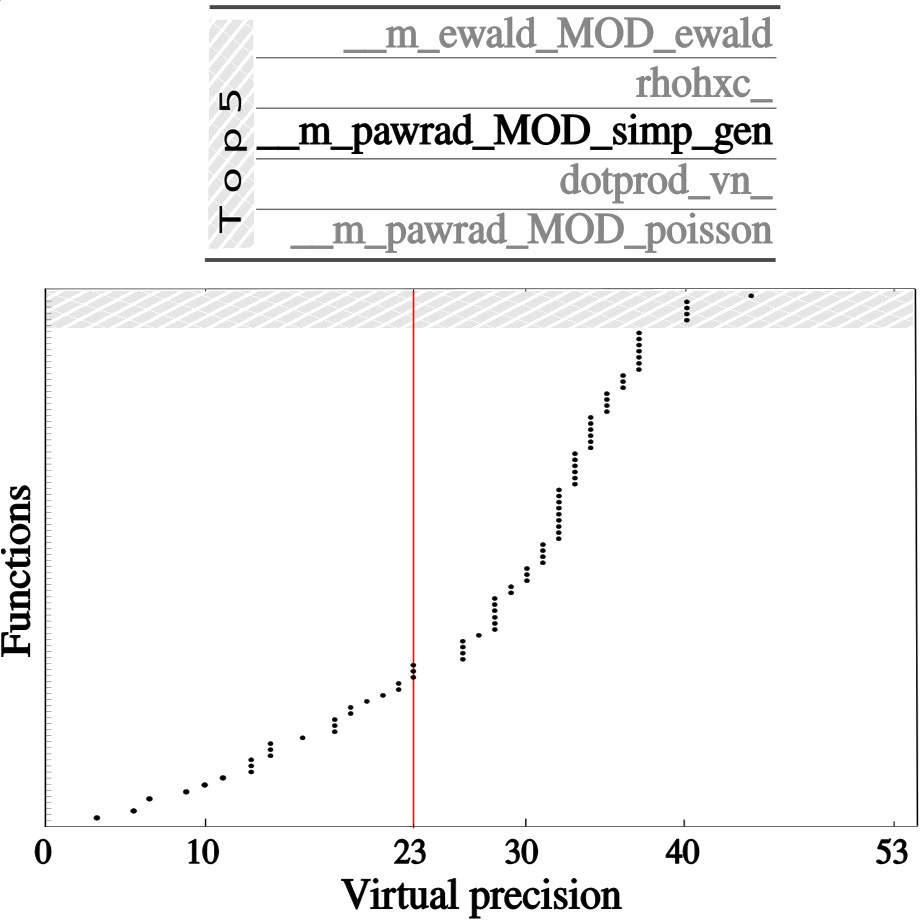
\includegraphics[width=\linewidth,height=6.5cm]{precision_perovskite_ABIDEV_2.png}
\end{minipage}
\hfill
\begin{minipage}{.475\linewidth}
\begin{alertblock}{Functions below 23bits}
\begin{itemize}
\item are more resistant
\item can potentially be changed to single precision
\end{itemize}
\end{alertblock}
\begin{alertblock}{Functions above 23bits}
\begin{itemize}
\item are less resistant
\item require further analyses
\end{itemize}
\end{alertblock}
\begin{alertblock}{Interesting function among the top 5}
\texttt{\_\_m\_pawrad\_MOD\_simp\_gen}
\end{alertblock}
\end{minipage}
\end{figure}
\end{frame}

\metroset{block=fill}

\begin{frame}{Simp\_gen: Evaluation with Veritracer}
\begin{block}{Computes an integral by Simpsons’ rule over a generalized 1D-grid}
\begin{itemize}
\item Can be seen as a \alert{dot product}
\end{itemize}
\end{block}
\begin{figure}
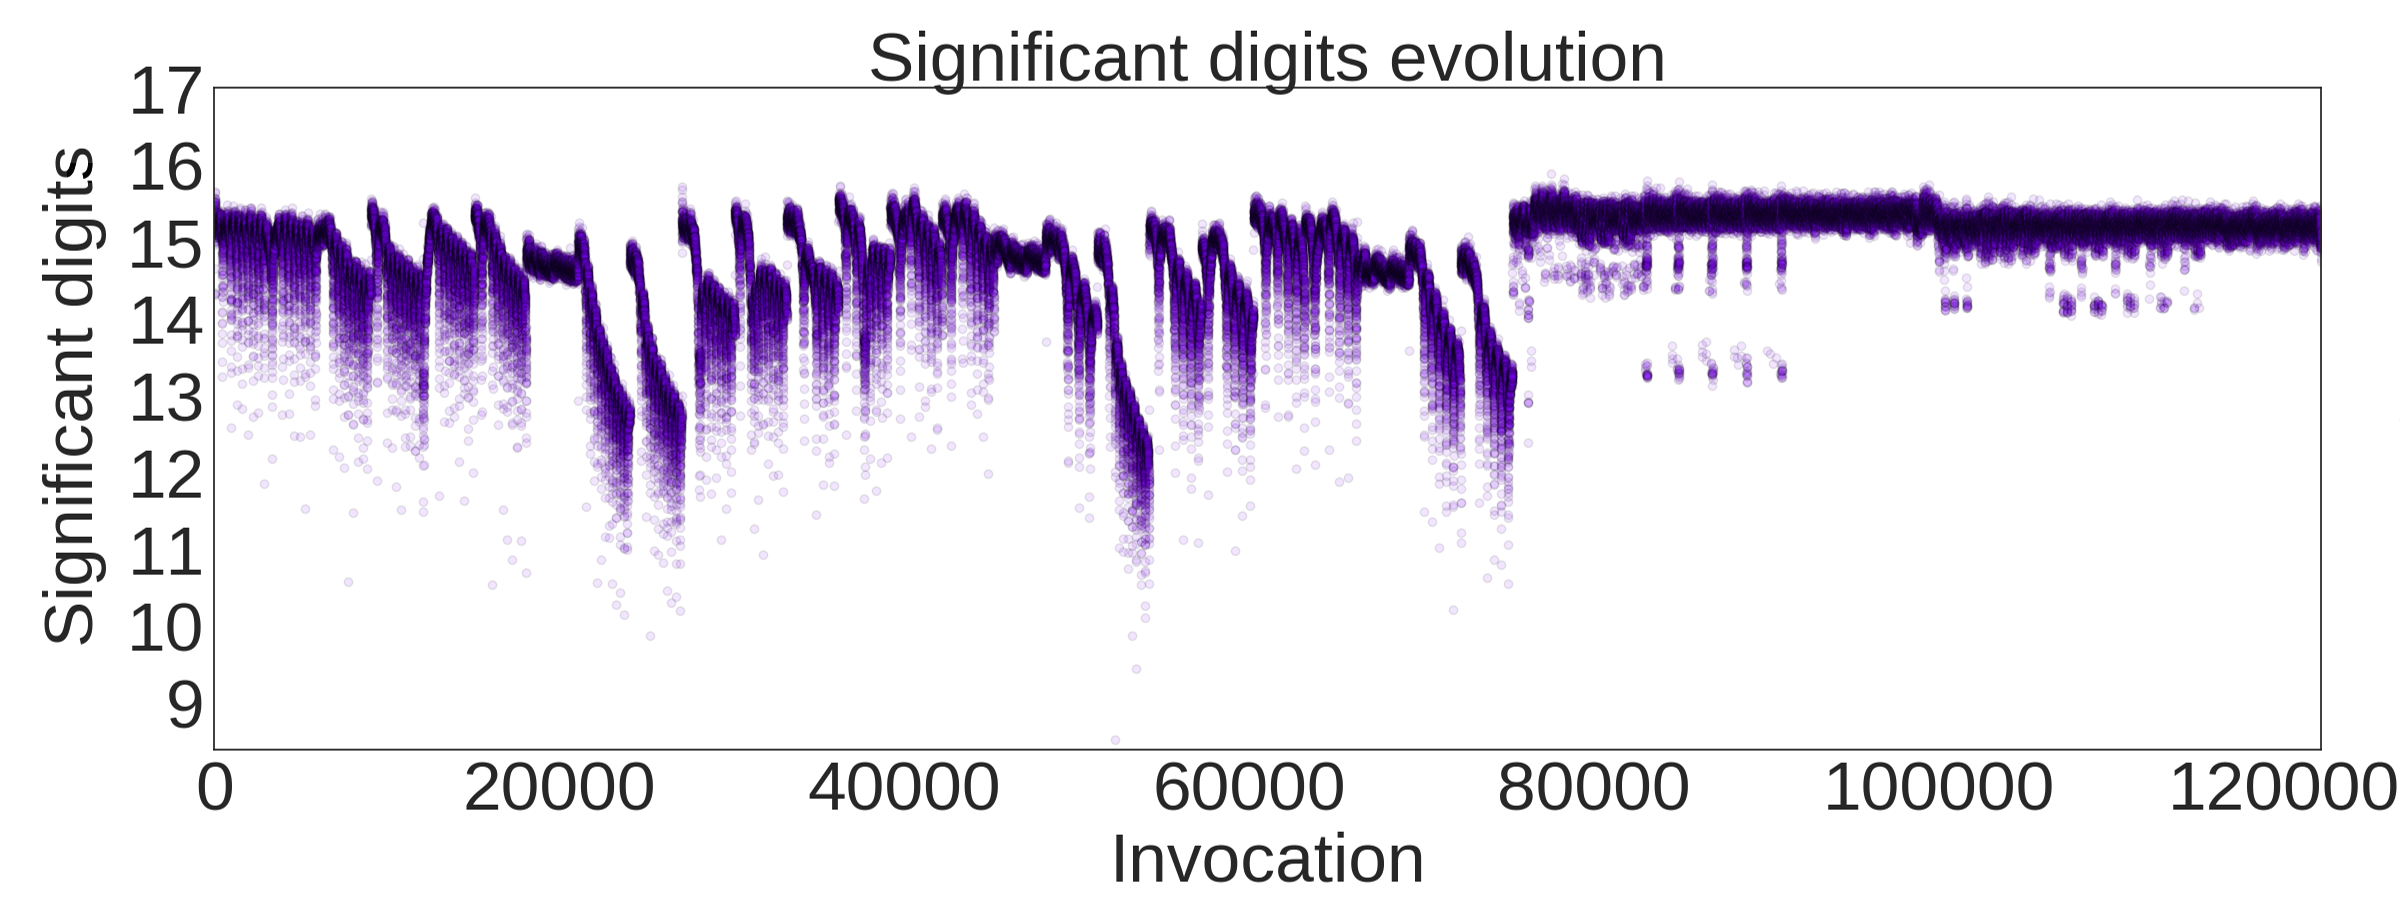
\includegraphics[width=\linewidth]{figure_1.png}
\caption{Evolution of the value returned by simp\_gen
with $t=53$ in Random Rounding mode 
with 24 samples in parallel on the \textbf{CINES Occigen} cluster 
(2106 nodes x2 Intel 12-Cores (E5-2690V3@2.6 GHz))}
\end{figure}
\end{frame}

\begin{frame}{Simp\_gen: the importance of the context analysis}
\begin{block}{}
\begin{itemize}
\item \alert{Colors} represent the \alert{different CSPs}
\item Red arrow seems to point an enhancement of the quality ...
\item ... but red points come from another context
\end{itemize}
\end{block}
\begin{figure}
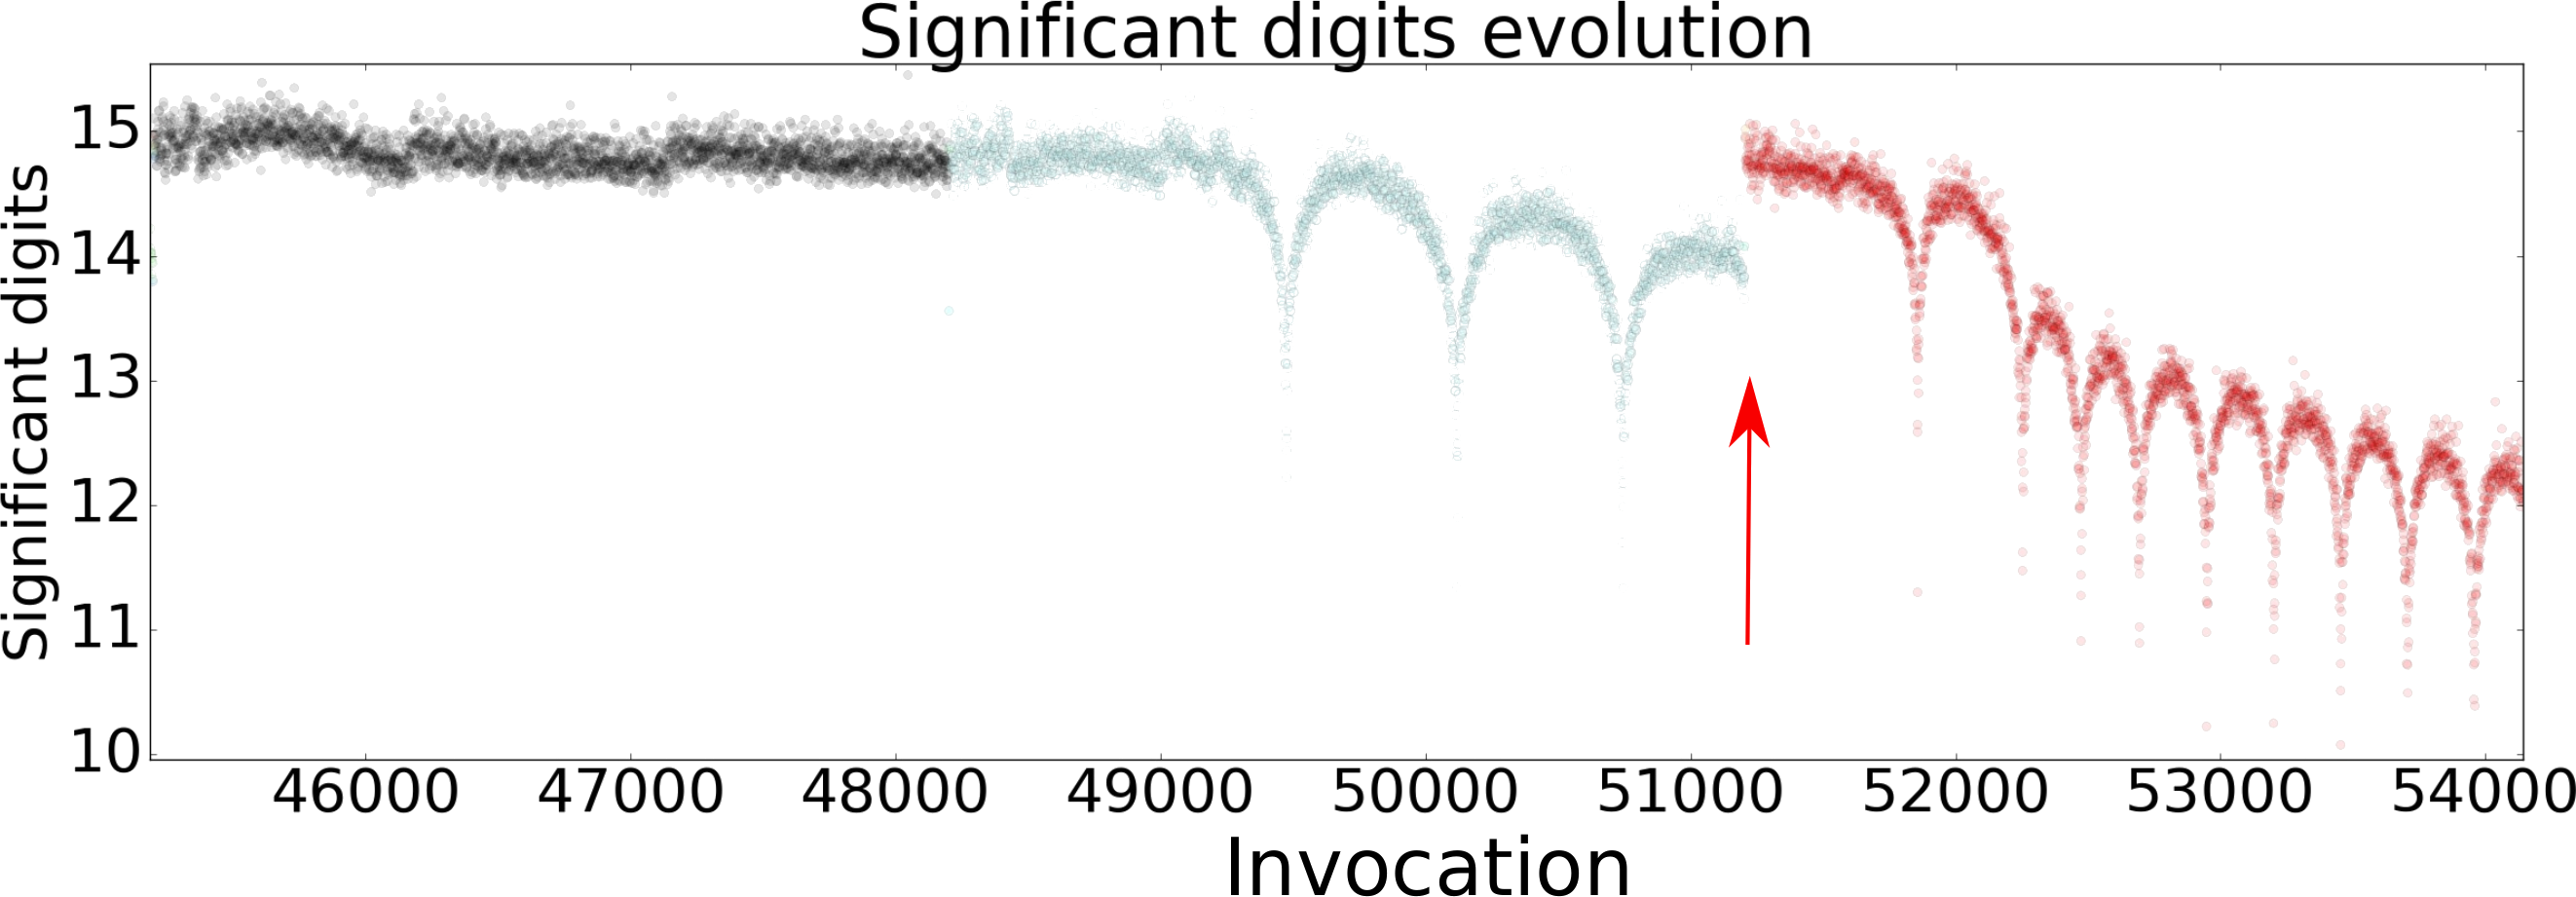
\includegraphics[width=\linewidth]{context-sensitive.png}
\end{figure}
\end{frame}

\begin{frame}{Simp\_gen: the importance of the context analysis}
\begin{block}{}
\begin{itemize}
\item \alert{Colors} represent the \alert{different CSPs}
\item Red arrow seems to point an enhancement of the quality ...
\item ... but red points come from another context
\item Hence the importance of separating contexts
\end{itemize}
\end{block}
\begin{figure}
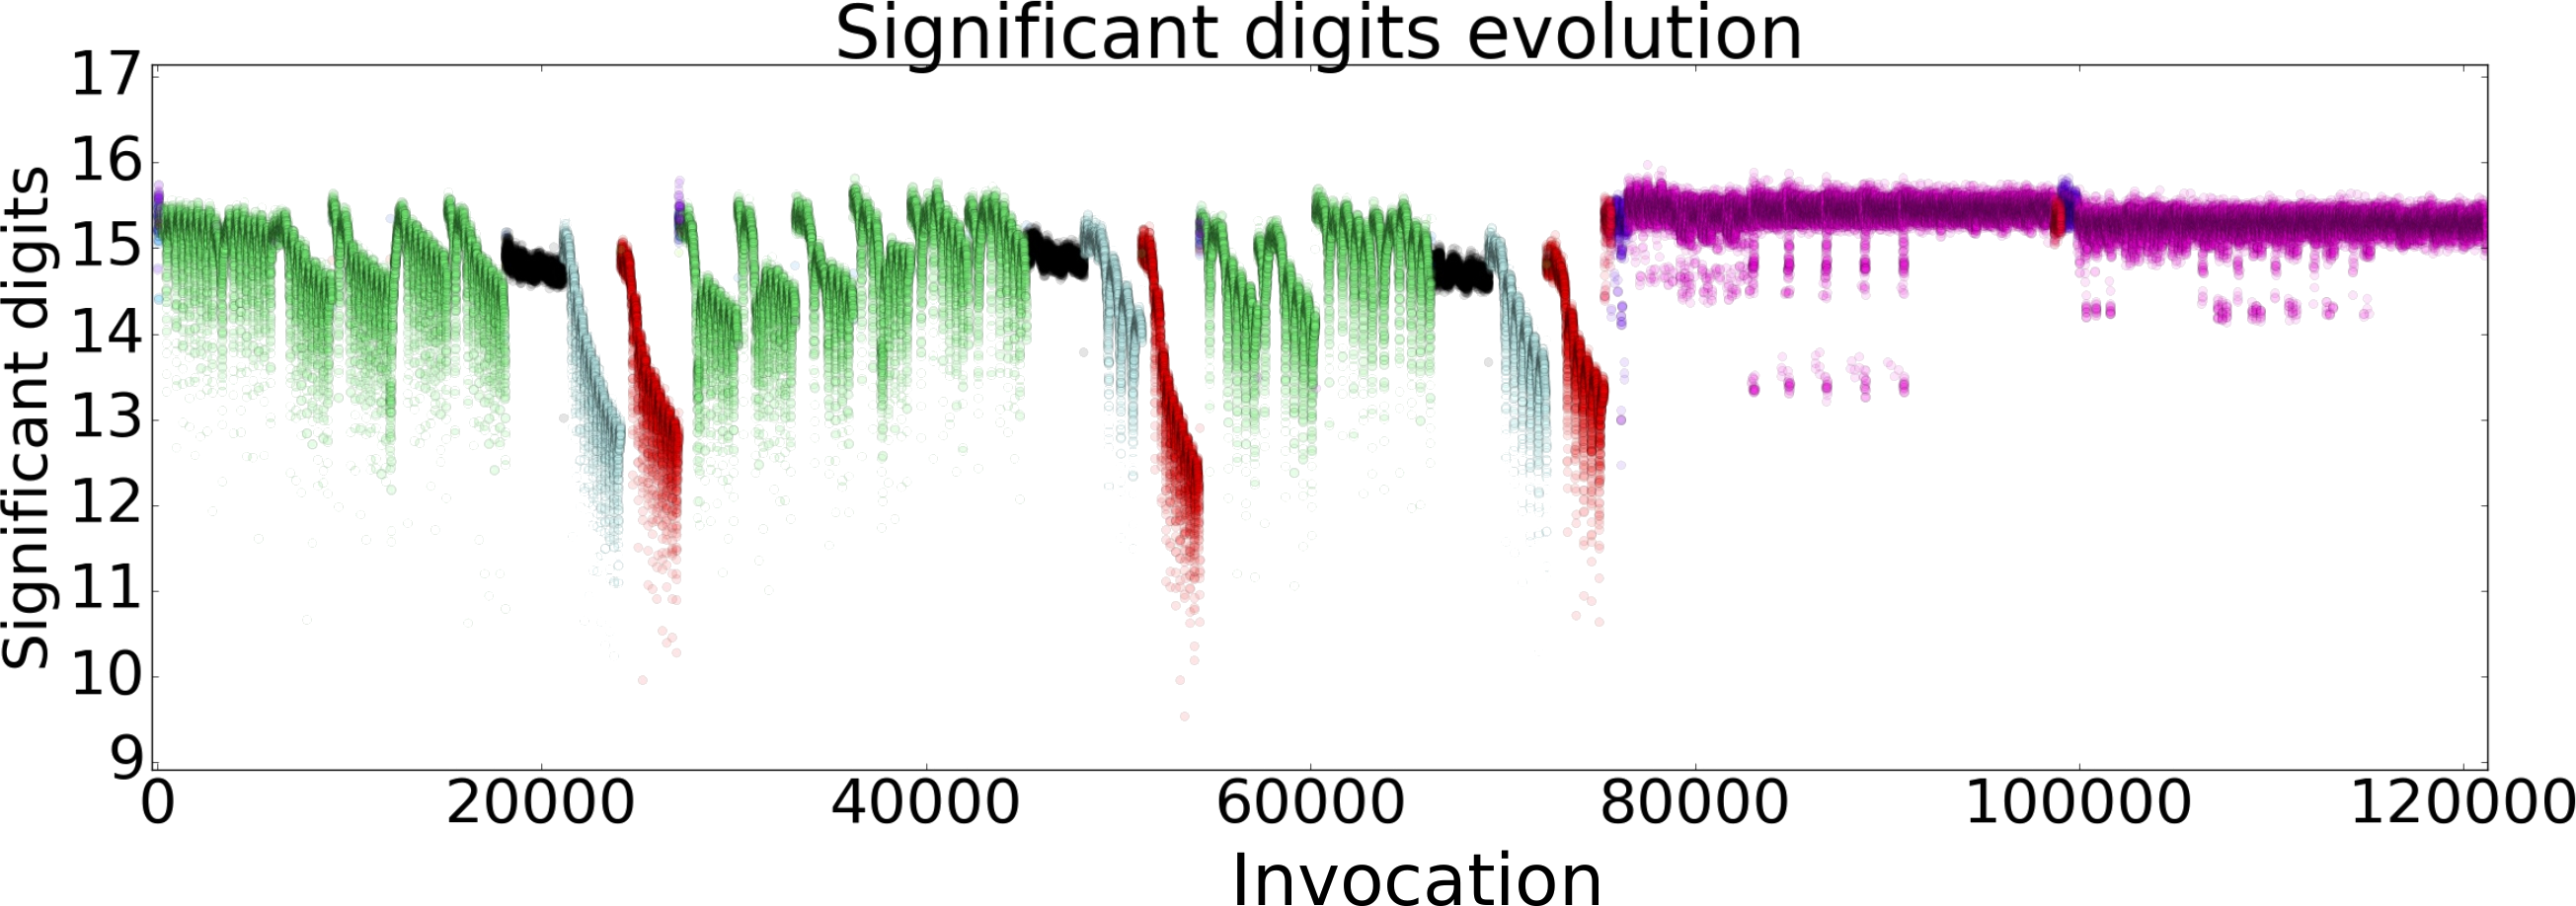
\includegraphics[width=\linewidth]{simp_gen_53_1.png}
\end{figure}
\end{frame}

% \begin{frame}[fragile]{Simp\_gen code}
% \begin{block}{Computes an integral by Simpsons’ rule over a generalized 1D-grid}
% \begin{itemize}
% \item Can be seen as a \alert{dot product}
% \item Replace by a compensated version (Dot2~\cite{ogita2005accurate})
% \item Implements with libeft~\cite{libeft}
% \end{itemize}
% \end{block}
% \begin{scriptsize}
% \begin{figure}
% \hspace{-.5cm}\begin{minipage}{.4\linewidth}
% \begin{minted}{fortran}
% subroutine simp_gen(intg,func,simfact)
% ...
% simp=zero
% do i=1,nn
%     simp=simp+func(i)*simfact(i)
% end do
% ...
% intg=simp+resid
% end subroutine
% \end{minted}
% \end{minipage}
% % \caption{Original code}
% \hspace{1.5cm}
% \begin{minipage}{.4\linewidth}
% \begin{minted}{fortran}
% subroutine simp_gen(intg,func,simfact)
% ...
% simp=zero

% call Dot2(intg,nn,func,simfact)

% ...
% intg=simp+resid
% end subroutine
% \end{minted}
% \end{minipage}
% % \caption{Compensated code}
% \end{figure}
% \end{scriptsize}
% \end{frame}

\begin{frame}[fragile]{Simp\_gen: A compensated version}
\metroset{block=fill}
% \begin{block}{Computes an integral by Simpsons' rule over a generalized 1D-grid}
% \begin{itemize}
% \item Can be seen a \alert{dot product}
% \item Replaces by a compensated version \alert{Dot2}~\cite{ogita2005accurate}
% \item The precision of \alert{30/31} CSPs is \alert{improved}
% \item 1 CSP has a low precision due to reentrance of the error
% \end{itemize}
% \end{block}
\hspace{-.35cm}\begin{minipage}{.59\linewidth}
\begin{figure}
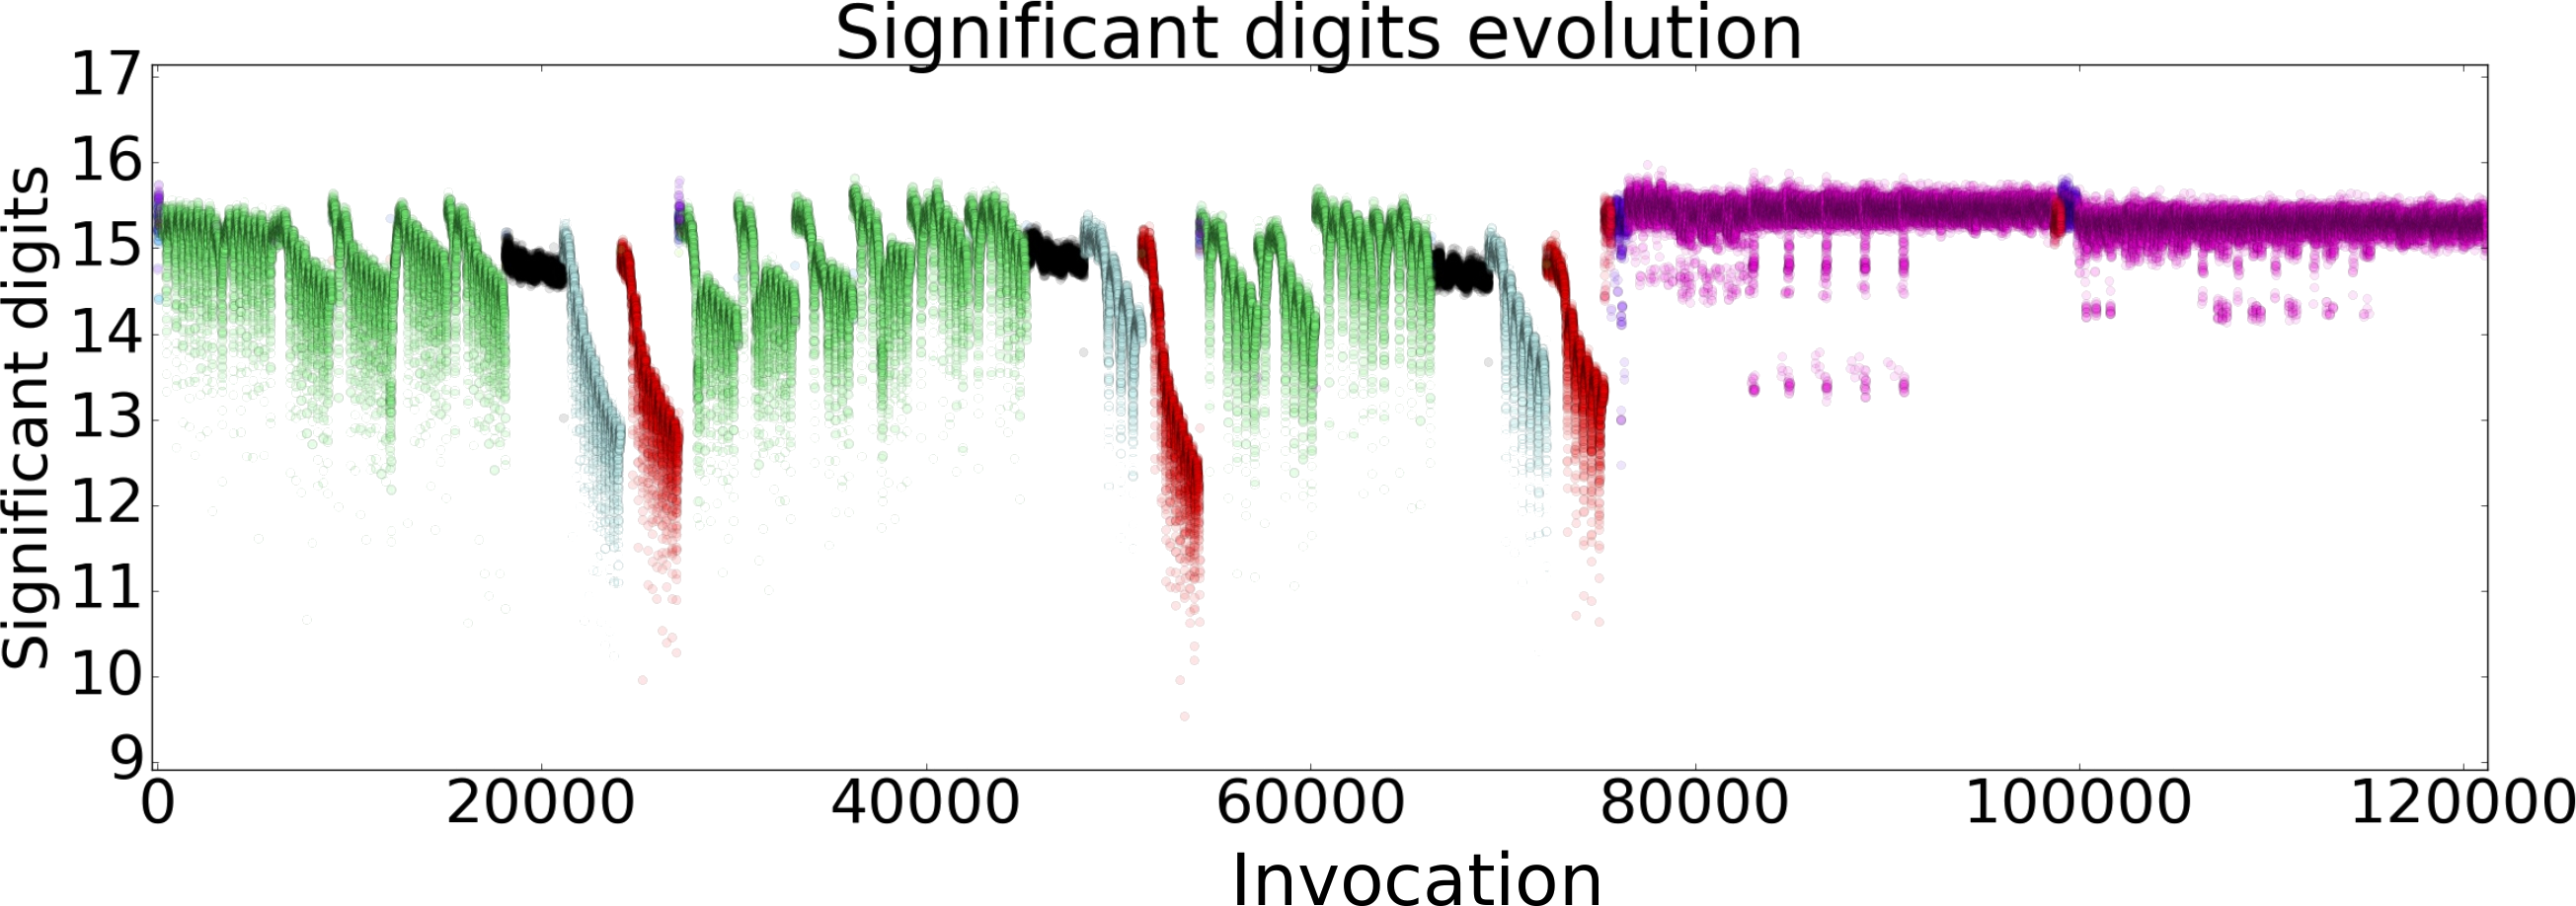
\includegraphics[width=\linewidth]{simp_gen_53_1.png}
\end{figure}
\begin{figure}
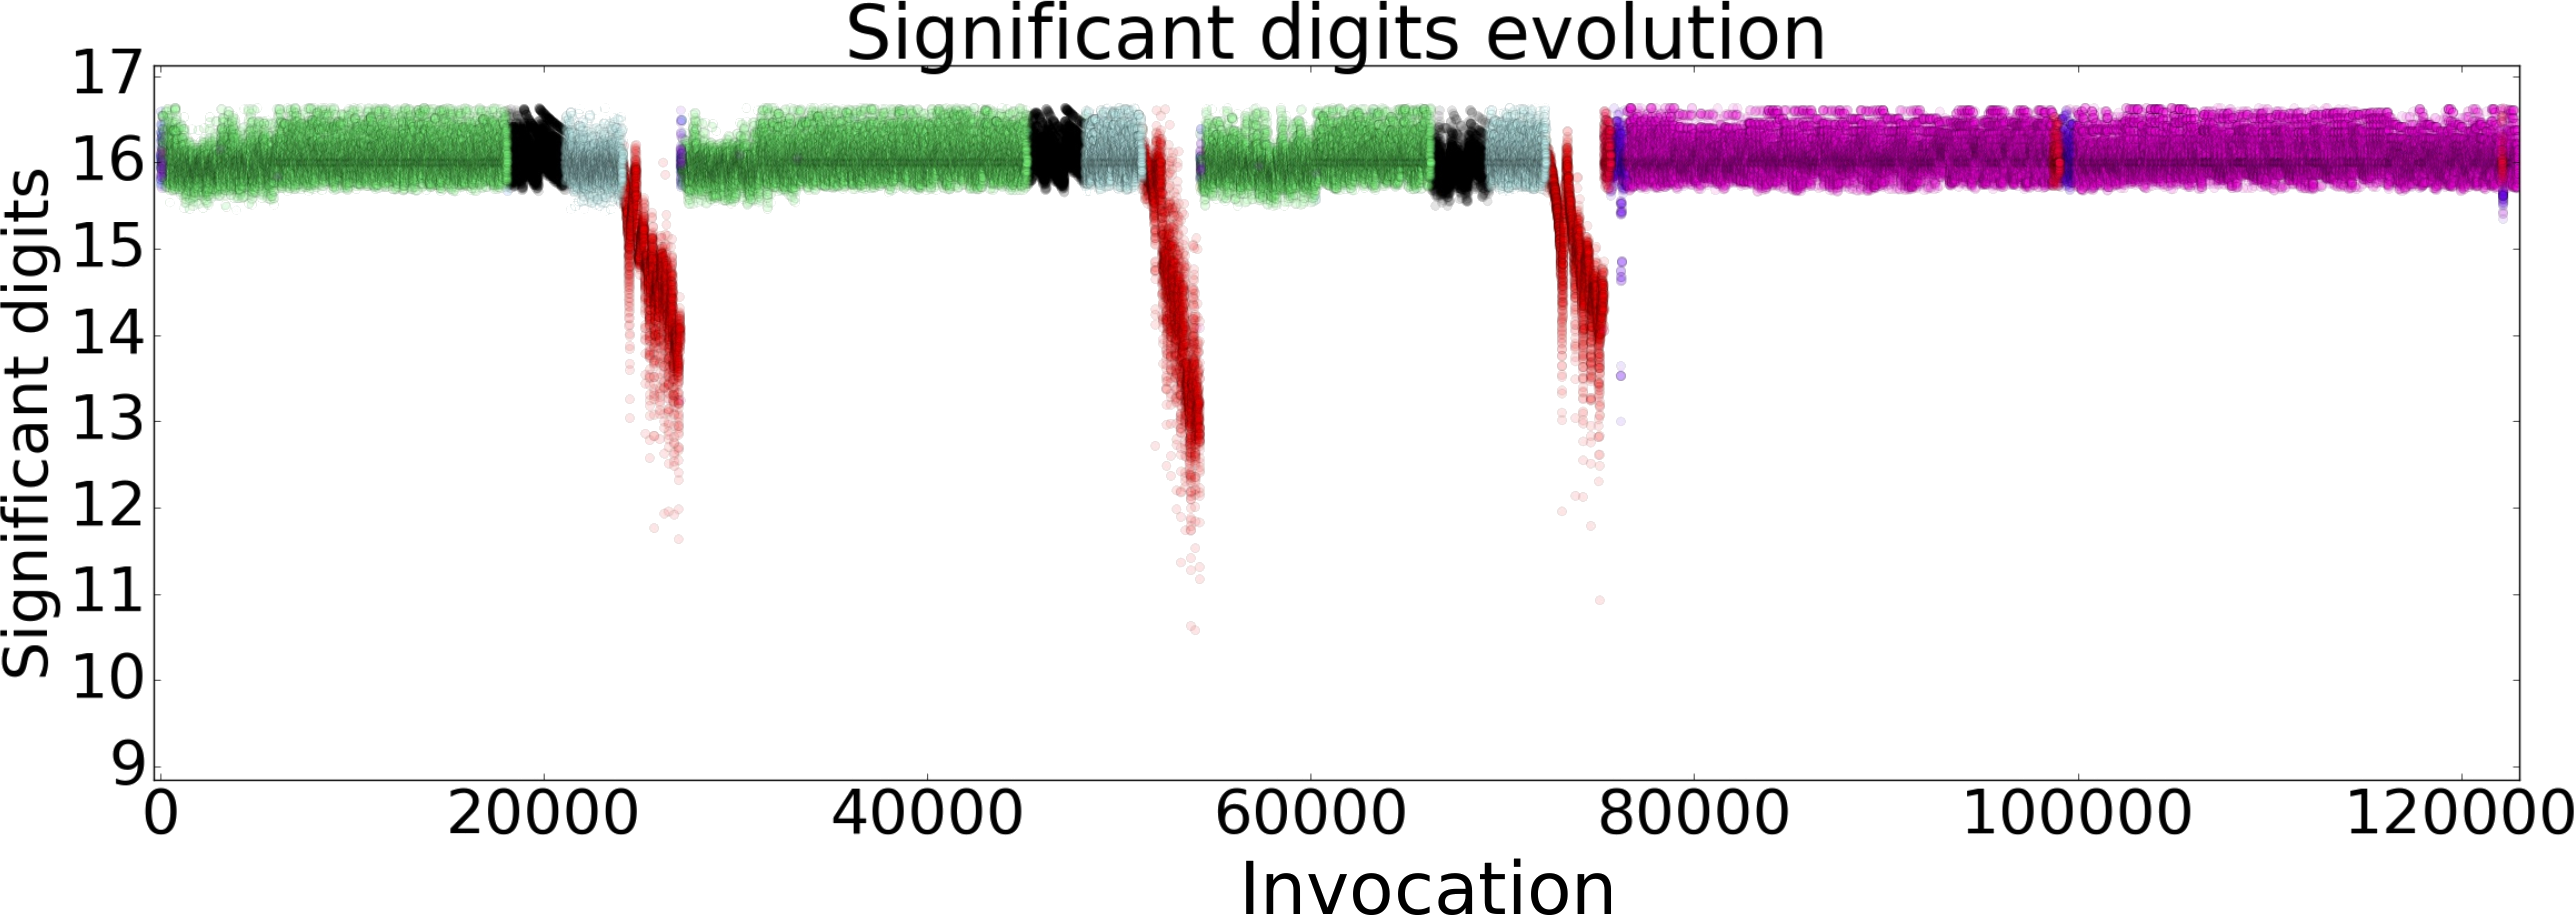
\includegraphics[width=\linewidth]{simp_gen_53_comp.png}
\end{figure}
\end{minipage}
\hspace{.25cm}
\begin{minipage}{.40\linewidth}
\begin{footnotesize}
\begin{block}{Simp\_gen: Altered version}
\begin{itemize}
\item Can be seen a \alert{dot product}
\item Replaces by a compensated version \alert{Dot2}~\cite{ogita2005accurate}
\item Implemented with \texttt{libeft}~\cite{libeft}
\item The precision of \alert{30/31} CSPs is \alert{improved}
\item 1 CSP has a low precision due to reentrance of the error
\end{itemize}
\end{block}
\end{footnotesize}
\end{minipage}
\end{frame}

\section{Conclusion}

\begin{frame}[fragile]{Conclusion}
\begin{small}
\begin{block}{Veritracer is a numerical debugger/optimizer which}
\begin{itemize}
\item Automatically \alert{instruments} codes through the verificarlo framework
\item Automatically \alert{plots} the \alert{temporal} numerical quality of variables
\item \alert{Provides contextual information} % with the Information Flow Analysis for a better understanding of interactions between variables
\end{itemize}
\end{block}
\begin{block}{Veritracer can be used on real world HPC applications to}
\begin{itemize}
\item \alert{Detect} the numerical sensitivity of functions
\item \alert{Classify} functions according to their numerical sensitivity
\item \alert{Observe} the numerical behavior of functions over time 
\end{itemize}
\end{block}
\end{small}
\end{frame}

\begin{frame}{Thank you for your attention}
\begin{figure}
% 
\includegraphics[scale=.5]{verificarlo-logo.pdf}
\hspace{1cm}

\includegraphics[scale=.4]{veritracer-logo.png}
\end{figure}
\vfill
Available on github:

\url{github.com/verificarlo/verificarlo}
\url{github.com/verificarlo/verificarlo/tree/veritracer}
\end{frame}

\appendix

% \begin{frame}[fragile]{Random Rounding mode (MCA)}
% \begin{figure}
% 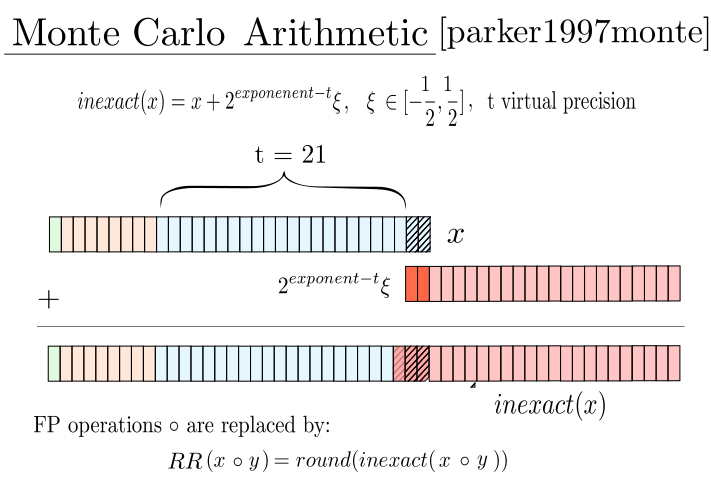
\includegraphics[scale=.5]{mca_model_RR.png}
% \end{figure}
% \end{frame}

% \begin{frame}[fragile]{Full MCA mode}
% \begin{figure}
% 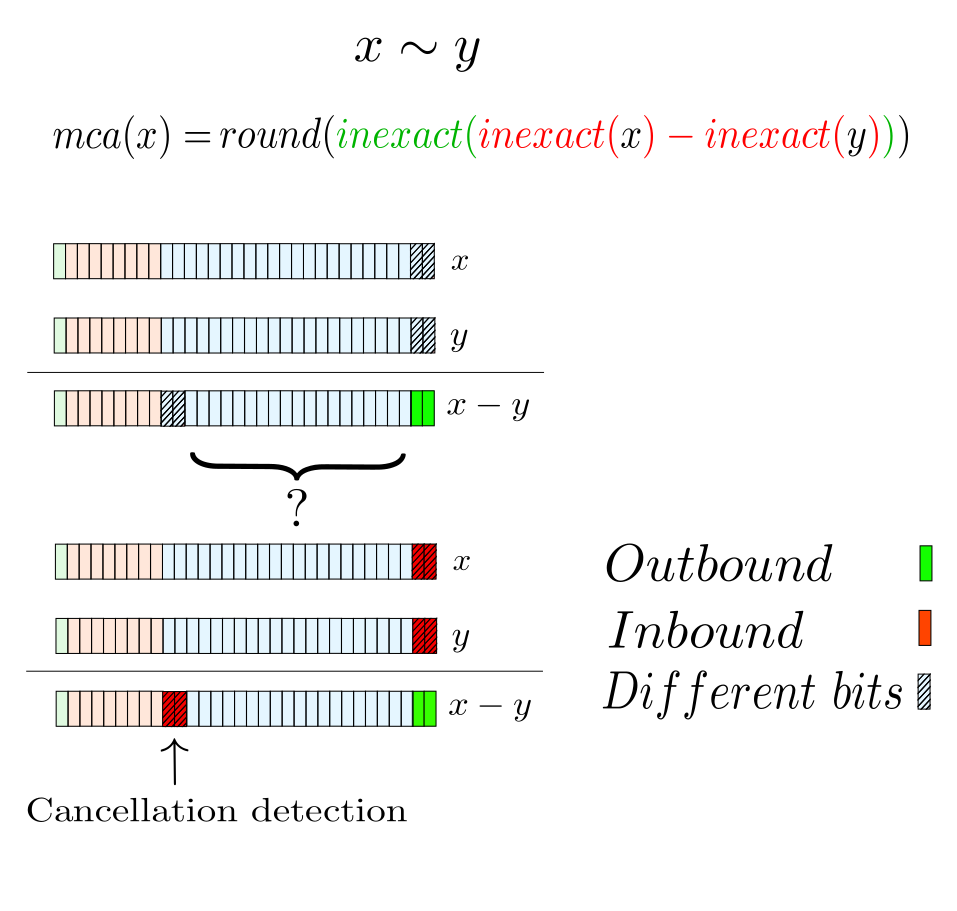
\includegraphics[scale=0.35]{inbound_outbound.png}
% \end{figure}
% \end{frame}

% \begin{frame}[fragile]{Bitmask backend}
% \begin{figure}
% 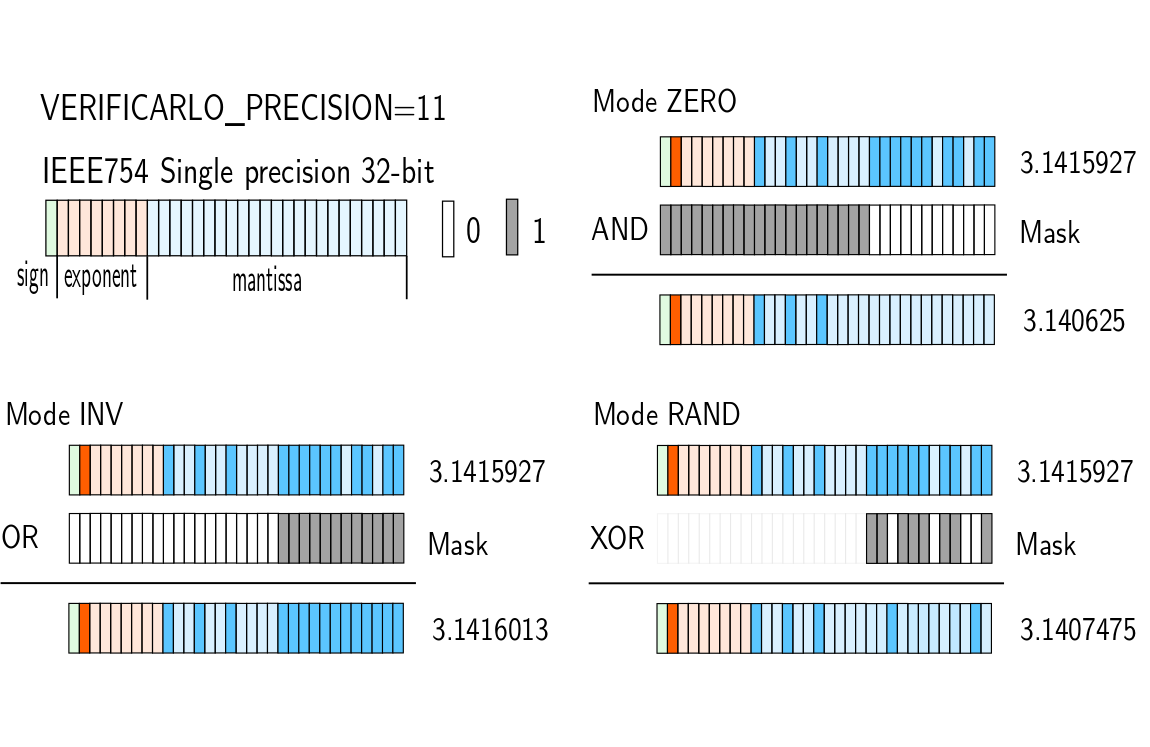
\includegraphics[width=\linewidth]{bitmask_portrait.png}
% \end{figure}
% \end{frame}

% \begin{frame}[fragile]{Errors propagation}
% \begin{figure}
% 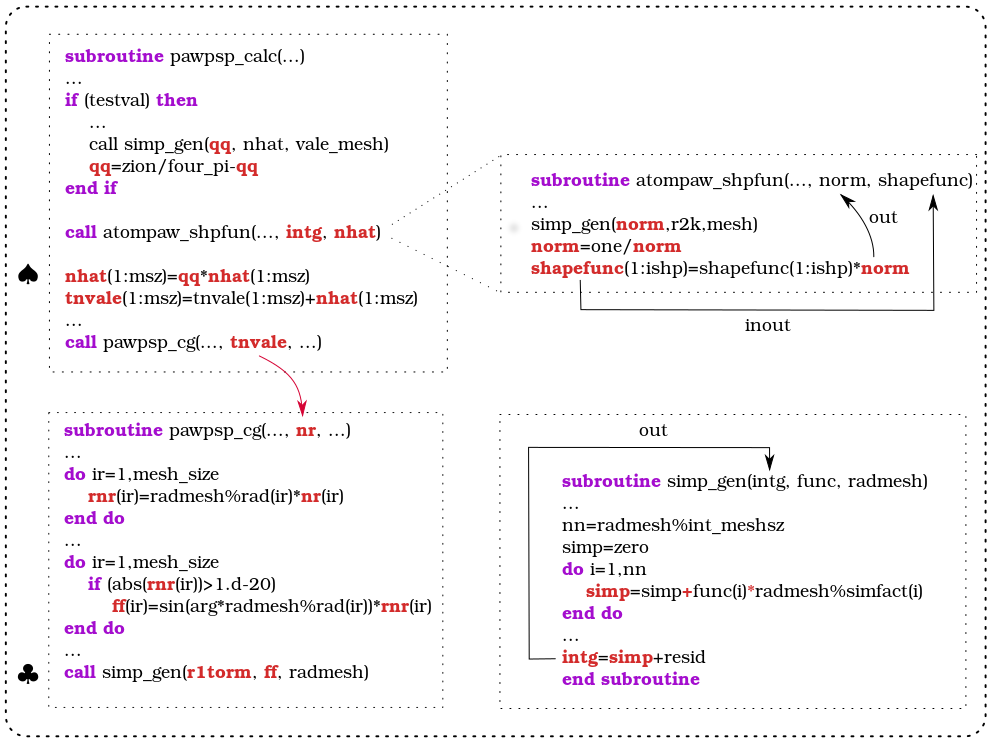
\includegraphics[scale=0.35]{error_propagation.png}
% \end{figure}
% \end{frame}

% % \begin{frame}{Simp\_gen: a zoom}
% % \begin{block}{Arch profile}
% % \begin{itemize}
% % \item Integral is calculated on a sinusoidal domain
% % \item Precision falls correspond to values close to 0
% % \item Which gives this arch profile
% % \end{itemize}
% % \end{block}
% % \begin{figure}
% % 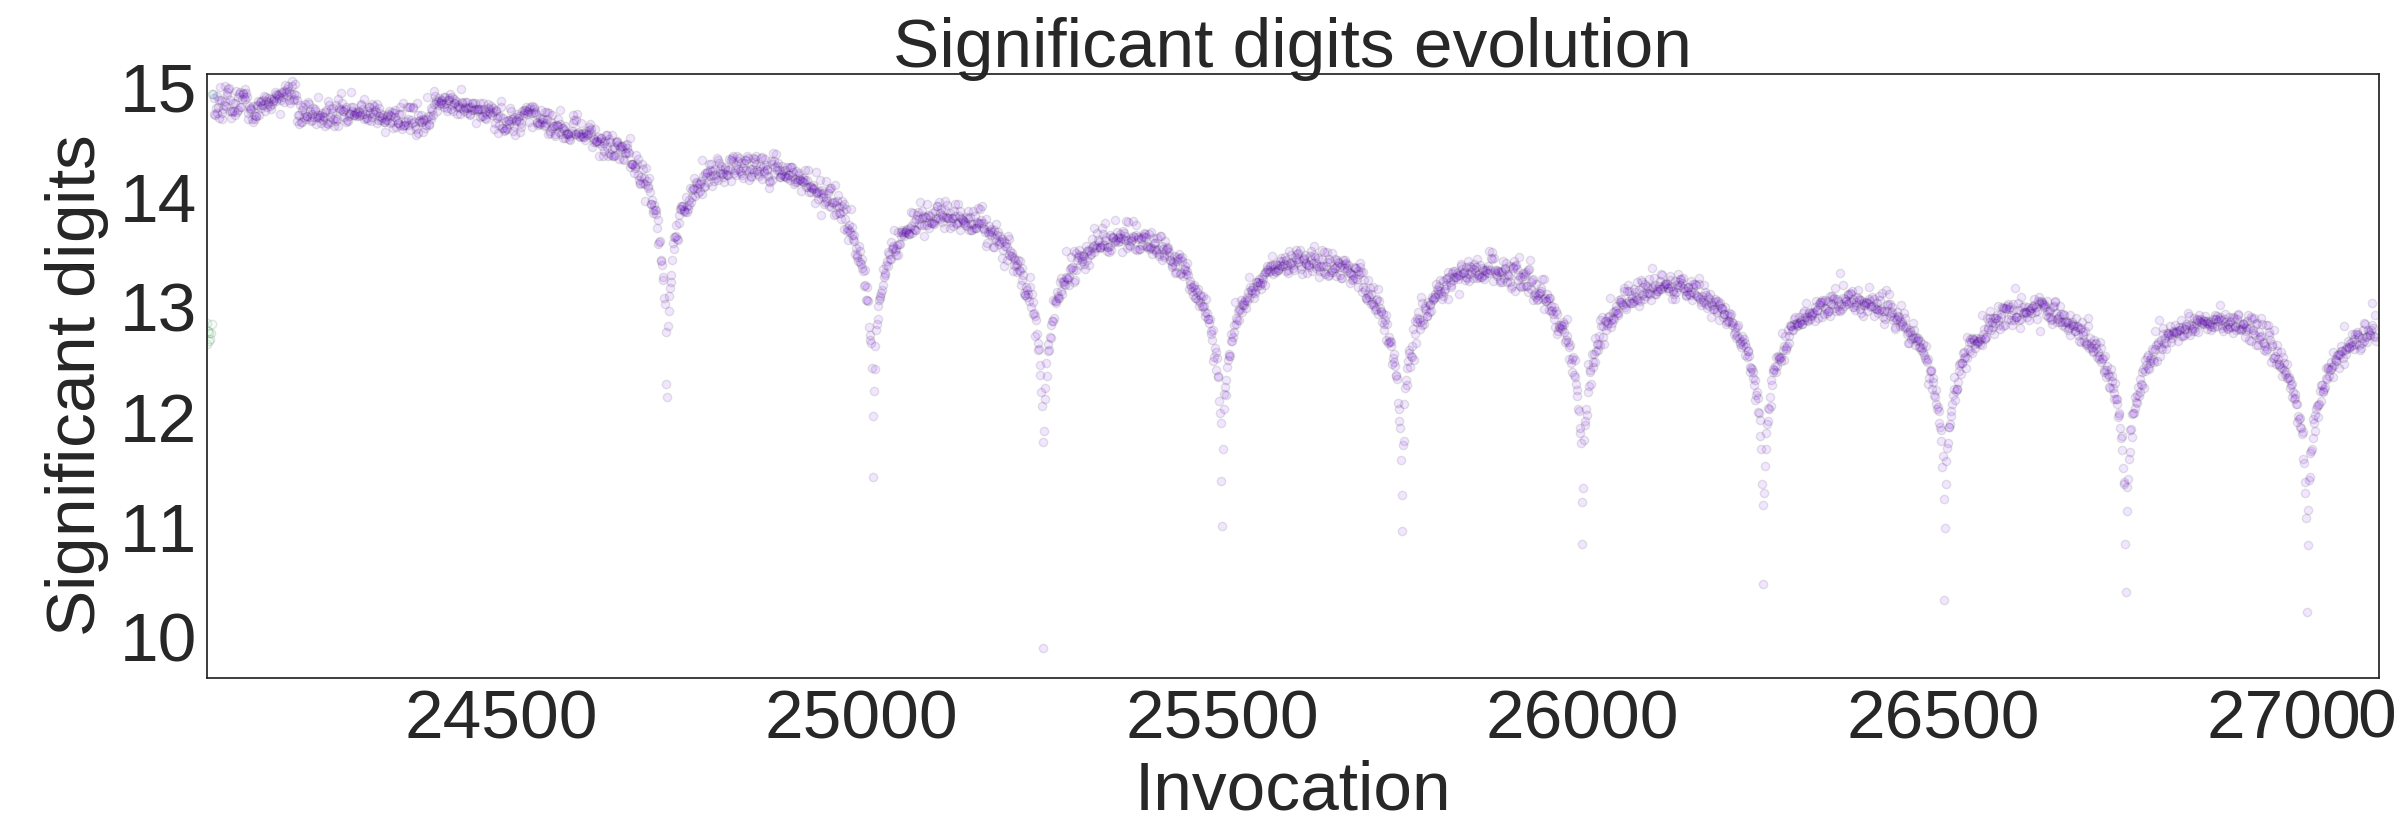
\includegraphics[width=\linewidth]{zoom.png}
% % \end{figure}
% % \end{frame}

% \begin{frame}[fragile]{Veritracer: the LLVM IR}
% \begin{tiny}
% \begin{minted}[frame=single]{c}
% void twoSum
% (double a, double b, double *x_ptr, double *err_ptr) {
%   double x = a + b;
%   double z = x - a;
%   double e = (a - (x - z)) + (b - z);
%   *x_ptr = x;
%   *err_ptr = e;
% }
% \end{minted}
% \begin{minipage}[c]{0.45\linewidth}
% \begin{minted}[resetmargins,frame=single, xrightmargin=-17pt]{llvm}
% define void @twoSum
% (float %a, float %b, float* %x_ptr, float* %e_ptr)
% {
%   %5 = load float* %a         ; 
%   %6 = load float* %b         ; 
%   %7 = fadd float %5, %6      ;     a+b
%   store float %7, float* %x   ; x = a+b 
%   %8 = load float* %x         ; 
%   %9 = load float* %a         ;
%   %10 = fsub float %8, %9     ;     x-a
%   store float %10, float* %z  ; z = x-a
%   %11 = load float* %a        ;       
%   %12 = load float* %x        ;
%   %13 = load float* %z        ;
%   %14 = fsub float %12, %13   ;     x-z
%   %15 = fsub float %11, %14   ;     a-(x-z)
%   %16 = load float* %b        ;
%   %17 = load float* %z        ; 
%   %18 = fsub float %16, %17   ;     b-z 
%   %19 = fadd float %15, %18   ;     a-(x-z)+(b-z)
%   store float %19, float* %e  ; e = a-(x-z)+(b-z)
%   %20 = load float* %x        ;
%   %21 = load float** %3       ;
%   store float %20, float* %21 ; *x_ptr = x
%   %22 = load float* %e        ;
%   %23 = load float** %4,      ; 
%   store float %22, float* %23 ; *e_ptr = e
%   ret void
% }
% \end{minted}
% \end{minipage}
% \hspace{.5cm}\begin{minipage}[b]{.45\linewidth}
% \begin{minted}[resetmargins,frame=single,xrightmargin=-30pt,xleftmargin=5pt]{llvm}
% define void @twoSum 
% (float %a, float %b, float* %x_ptr, float* %err_ptr) 
% {
%   %1 = fadd float %a, %b        ; a+b     (x)
%   %2 = fsub float %1, %a        ; (a+b)-a (z)
%   %3 = fsub float %1, %2        ; x-z  
%   %4 = fsub float %a, %3        ; a-(x-z)
%   %5 = fsub float %b, %2        ; b-z
%   %6 = fadd float %5, %4        ; (b-z)+(a-(x-z)) 
%   store float %1, float* %x_ptr ; *x_ptr = x
%   store float %6, float* %e_ptr ; *e_ptr = e
%   ret void
% }
% \end{minted}
% \end{minipage}
% \end{tiny}
% \end{frame}

% \begin{frame}{Reducing the search space}
% \metroset{block=fill}
% \begin{alertblock}{Instrumenting one function of the program at a time}
% \begin{itemize}
% \item Executes each version with the maximal MCA error 
% \item Compares the MCA computed value with the reference:
% \begin{description}
% \item[\alert{Different}]: the function is tagged as \alert{critical}
% \item[\alert{Identical}]: the function is tagged \alert{not critical}
% \end{description}
% \end{itemize}
% \end{alertblock}
% \begin{figure}
% 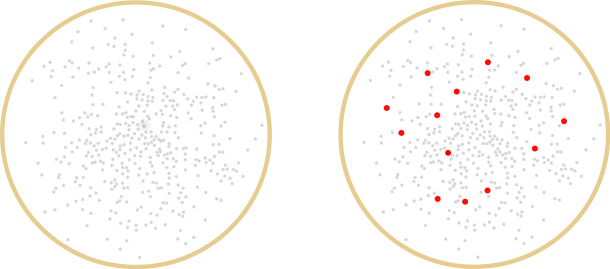
\includegraphics[width=.75\linewidth]{reduction.png}
% \end{figure}
% \begin{center}
% \begin{large}
% 2952 function $\Rightarrow$ 88 functions \\
% Reduces the search space by \alert{$\mathbf{\times 30}$}
% \end{large}
% \end{center}
% \end{frame}

% \begin{frame}{Ordering the search space}
% \metroset{block=fill}
% \begin{alertblock}{Problem}
% Functions do not have the same numerical behavior: some functions \alert{are less sensitive to numerical errors than others}
% \end{alertblock}
% \begin{alertblock}{Idea}
% Classifying functions according to their 
% \alert{numerical stress resistance}
% \end{alertblock}
% \begin{figure}
% \only<1>{
\includegraphics[width=.75\linewidth, height=5cm]{ordering.png}}
% \only<2>{
\includegraphics[width=.75\linewidth, height=5cm]{ordering_simp_gen.png}}
% \end{figure}
% \end{frame}

\begin{frame}[allowframebreaks]{References}

  \bibliography{demo}
  \bibliographystyle{abbrv}

\end{frame}

\end{document}
